\documentclass{wissdoc}
% Autor: Roland Bless 1996-2009, bless <at> kit.edu
% ----------------------------------------------------------------
% Hauptdokument
% ----------------------------------------------------------------
%%
%% $Id: thesis.tex 65 2012-05-10 10:32:11Z bless $
%%
%
% Zum Erstellen zweiseitiger PDFs (für Buchdruck) in der Datei "wissdoc.cls" folgende Zeile abändern:
%
% \LoadClass[a4paper,12pt,oneside]{book} % diese Klasse basiert auf ``book''
% in
%\LoadClass[a4paper,12pt,titlepage]{book} % diese Klasse basiert auf ``book''
%
%
% wissdoc Optionen: draft, relaxed, pdf --> siehe wissdoc.cls
% ------------------------------------------------------------------
% Weitere packages: (Dokumentation dazu durch "latex <package>.dtx")
\usepackage[numbers,sort&compress]{natbib}
% \usepackage{varioref}
% \usepackage{float}    %z.B. \floatstyle{ruled}\restylefloat{figure}
% \usepackage{subfigure}
% \usepackage{fancybox} % für schattierte,ovale Boxen etc.
% \usepackage{tabularx} % automatische Spaltenbreite
% \usepackage{supertab} % mehrseitige Tabellen
% \usepackage[svnon,svnfoot]{svnver} % SVN Versionsinformation 
\usepackage{amsmath,amsthm,amssymb}
\usepackage[ruled,vlined,linesnumbered]{algorithm2e}
\usepackage{graphicx}
\usepackage{hyperref}
\usepackage{makecell}
\usepackage{pgfplots}
\usepackage{verbatim}
\usepackage[width=.75\textwidth]{caption}
\usepackage{listings}
%% ---------------- end of usepackages -------------

\colorlet{punct}{red!60!black}
\definecolor{background}{HTML}{EEEEEE}
\definecolor{delim}{RGB}{20,105,176}
\colorlet{numb}{magenta!60!black}

\lstdefinelanguage{json}{
    basicstyle=\scriptsize\ttfamily,
    numbers=left,
    numberstyle=\scriptsize,
    stepnumber=1,
    numbersep=8pt,
    showstringspaces=false,
    breaklines=true,
    frame=lines,
    backgroundcolor=\color{background},
    literate=
     *{0}{{{\color{numb}0}}}{1}
      {1}{{{\color{numb}1}}}{1}
      {2}{{{\color{numb}2}}}{1}
      {3}{{{\color{numb}3}}}{1}
      {4}{{{\color{numb}4}}}{1}
      {5}{{{\color{numb}5}}}{1}
      {6}{{{\color{numb}6}}}{1}
      {7}{{{\color{numb}7}}}{1}
      {8}{{{\color{numb}8}}}{1}
      {9}{{{\color{numb}9}}}{1}
      {:}{{{\color{punct}{:}}}}{1}
      {,}{{{\color{punct}{,}}}}{1}
      {\{}{{{\color{delim}{\{}}}}{1}
      {\}}{{{\color{delim}{\}}}}}{1}
      {[}{{{\color{delim}{[}}}}{1}
      {]}{{{\color{delim}{]}}}}{1},
}

%\svnversion{$Id: thesis.tex 65 2012-05-10 10:32:11Z bless $} % In case that you want to include version information in the footer

%% Informationen für die PDF-Datei
\hypersetup{
 pdfauthor={Benedikt Lüken-Winkels},
 pdftitle={Masterarbeit}
 pdfsubject={Untersuchungen zur Henon Iteration},
 pdfkeywords={Masterarbeit}
}

% Macros, nicht unbedingt notwendig
\input{macros}

% Print URLs not in Typewriter Font
\def\UrlFont{\rm}

\newcommand{\blankpage}{% Leerseite ohne Seitennummer, nächste Seite rechts
 \clearpage{\pagestyle{empty}\cleardoublepage}
}

%% Einstellungen für das gesamte Dokument

% Trennhilfen
% Wichtig! 
% Im ngerman-paket sind zusätzlich folgende Trennhinweise enthalten:
% "- = zusätzliche Trennstelle
% "| = Vermeidung von Ligaturen und mögliche Trennung (bsp: Schaf"|fell)
% "~ = Bindestrich an dem keine Trennung erlaubt ist (bsp: bergauf und "~ab)
% "= = Bindestrich bei dem Worte vor und dahinter getrennt werden dürfen
% "" = Trennstelle ohne Erzeugung eines Trennstrichs (bsp: und/""oder)

% Trennhinweise fuer Woerter hier beschreiben
\hyphenation{
% Pro-to-koll-in-stan-zen
}

% Index-Datei öffnen
\ifnotdraft{\makeindex}

\begin{document}

\frontmatter
\pagenumbering{roman}
\ifnotdraft{
 %% Titelseite
%% Vorlage $Id: titelseite.tex 61 2012-05-03 13:58:03Z bless $

\def\usesf{}
\let\usesf\sffamily % diese Zeile auskommentieren für normalen TeX Font

\newsavebox{\Erstgutachter}
\savebox{\Erstgutachter}{\usesf xxxxxxxxxx}
\newsavebox{\Zweitgutachter}
\savebox{\Zweitgutachter}{\usesf xxxxxxxxxx}
\newsavebox{\Betreuer}
\savebox{\Betreuer}{\usesf xxxxxxxxxx}

\begin{titlepage}
\setlength{\unitlength}{1pt}
\begin{picture}(0,0)(85,770)
%\includegraphics[width=\paperwidth]{logos/KIT_Deckblatt}
\end{picture}

\thispagestyle{empty}

%\begin{titlepage}
%%\let\footnotesize\small \let\footnoterule\relax
\begin{center}
\hbox{}
\vfill
{\usesf
{\huge\bfseries Implementierung nichtlinearer Taylormodelle \par}
\vskip 1.8cm
{\huge Forschungspraktikum}\\


{\large Universität Trier\\
FB IV - Informatikwissenschaften\\
Professur Arithmetische Algorithmen\\}

\vskip 3cm
\begin{tabular}{p{3cm}l}
Betreuer: & apl. Prof. Dr.  Norbert Müller \\
\end{tabular}
\vskip 3cm
Vorgelegt am xx.xx.xxxx von:\\
\vskip .5cm
Benedikt Lüken-Winkels\\
Baltzstraße 6\\
54296 Trier\\
s4beluek@uni-trier.de\\
Matr.-Nr. 1138844
}
\end{center}
\vfill
\end{titlepage}
%% Titelseite Ende


%%% Local Variables: 
%%% mode: latex
%%% TeX-master: "thesis"
%%% End: 

 %\blankpage % Leerseite auf Titelrückseite
 \chapter*{Zusammenfassung}
%% ==============================
In dieser Arbeit wurde die Verwendung nichtlinearer Taylormodelle in der Praxis anhand der zweidimensionalen H\e non-Abbildung untersucht. Die Anwendung spezieller Operationen auf den Taylormodellen und die Verwendung der reellen Zahlen der \verb+iRRAM+-Softwarebibliothek ergeben eine vielzahl an Konfigurationsmöglichkeiten, welche experimentell verglichen und evaluiert wurden, um eine möglichst optimale Belegung der Parameter zu finden.

Der Quellcode des im Zuge der Arbeit entstandenen Programms \verb+HOTM+ (\textit{High Order Taylor Model}) ist Online\footnote{\url{https://gitlab.rlp.net/s4beluek/hotaylormodels} (Stand 30.03.21)} und auf einem der Arbeit beigelegten Datenträger verfügbar.
  
}
%
%% *************** Hier geht's ab ****************
%% ++++++++++++++++++++++++++++++++++++++++++
%% Verzeichnisse
%% ++++++++++++++++++++++++++++++++++++++++++
\ifnotdraft{
{\parskip 0pt\tableofcontents} % toc bitte einzeilig
%\blankpage
\listoffigures
%\blankpage
\listoftables
%\blankpage
\lstlistoflistings
}


%% ++++++++++++++++++++++++++++++++++++++++++
%% Hauptteil
%% ++++++++++++++++++++++++++++++++++++++++++
\graphicspath{{img/}}

\mainmatter
\pagenumbering{arabic}
%% Einleitung.tex
%% $Id: einleitung.tex 61 2012-05-03 13:58:03Z bless $
%%

\chapter{Einleitung}
\label{ch:Einleitung}
%% ==============================
Die Einleitung besteht aus der Motivation, der Problemstellung, der Zielsetzung und einem erster Überblick über den Aufbau der Arbeit.

%% ==============================
\section{Motivation}
%% ==============================
\label{ch:Einleitung:sec:Motivation}

Warum ist das zu bearbeitende Themengebiet spannend und relevant?

%% ==============================
\section{Problemstellung}
%% ==============================
\label{ch:Einleitung:sec:Problemstellung}

Welches Problem/welche Probleme können in diesem Themengebiet identifiziert werden?

%% ==============================
\section{Zielsetzung}
%% ==============================
\label{ch:Einleitung:sec:Zielsetzung}

Was ist das Ziel der Arbeit. Wie soll das Problem gelöst werden?


%% ==============================
\section{Gliederung/Aufbau der Arbeit}
%% ==============================
\label{ch:Einleitung:sec:Gliederung}

Was enthalten die weiteren Kapitel? Wie ist die Arbeit aufgebaut? Welche Methodik wird verfolgt?  

\section{Relevante Literatur}
Die für diese Arbeit relevante Literatur lässt sich in vier Kategorien aufteilen, vergleichbar mit den später eingeführten Abstraktionsebenen, die sich aus dem Aufbau der \verb+HOTM+ ergeben. Für die grundlegende Zahlendarstellung wir die Implementierung der reellen Zahlen der \verb+iRRAM+ von Müller in \cite{Mller2009EnhancingIE}, beziehungsweise \cite{mueller2001} verwendet. Funktionsweisen und mögliche Anpassungen der Software-Bibilothek können diesen Quellen entnommen werden. Für eine theoretische Grundlage der hier praktisch angewendeten Berechenbaren Analysis wird auf ein Tutorial von Brattka \textit{et al} \cite{Brattka2008} verwiesen. Spandl untersucht in \cite{DBLP:spandl} mit Hilfe der \verb+iRRAM+ den Lyapunov Exponenten für dynamische Systeme und zieht dabei Intervallmethoden heran, was einen zentralen Teil dieser Arbeit darstellt. 

Da die \verb+HOTM+ auf der nächst höheren Ebene aus Polynomen mit Intervallkoeffizienten bestehen, wurde eine allgemeine Intervallarithmetik, wie im Standardwerk von Moore \cite{moore1979} beschrieben implementiert. Yan \textit{et al} führen in \cite{geobuckets} einen Algorithmus ein, der die Addition von Polynomen effizient gestaltet, welcher in \cite{geobucketsmulti} für die Multiplikation formuliert ist. Mit dieser Basis können die Taylormodelle, wie in \cite{makino2001} und \cite{DBLP:conf/macis/BrausseKM15} beschrieben, implementiert werden.

In \cite{DBLP:conf/macis/BrausseKM15} sind zudem weiterführende Operationen auf Taylormodellen zu finden. Diese werden unter anderem im Programm \verb+Tangentspace+, auf dem die \verb+HOTM+s aufbauen, verwendet und ermöglichen geometrische Lösungen für Konfliktgesteuerte Gleichungslöser. Die Funktionsweise der so implementierten Taylormodelle wird an Hand der H\e non-Abblildung untersucht. Hierzu existieren neben dem ursprünglichen Paper von M. H\e non \cite{henon1976}, viele Experimente und Untersuchungen, wie , sich mit verschiedenen Parameterbelegungen beschäftigen oder .






%%% Local Variables: 
%%% mode: latex
%%% TeX-master: "thesis"
%%% End: 
  % Einleitung
%% grundlagen.tex
%% $Id: grundlagen.tex 61 2012-05-03 13:58:03Z bless $
%%

\chapter{Grundlagen}
\label{ch:Grundlagen}
%% ==============================
\section{H\e non-Abbildung}
Die H\e non-Abbildung bietet eine Möglichkeit, das Verhalten eines seltsamen Attraktors (\textit{engl. \anf{strange attractor}}), wie dem des Lorenz Systems, mit einer recht einfachen Abbildung zu untersuchen.

Konviergieren die Werte einer Funktion in einem bestimmten Wertebereich $R$, der Fangzone (\textit{engl. \anf{trapping zone}}), gegen einen Punkt oder eine Kurve, spricht man von einem Attraktor. Dieser Attraktor kann jedoch auch eine komplexere Struktur haben. Auf einem solchen seltsamen Attraktor springen die Werte hin und her und reagieren hochempfindlich auf Änderungen der Initialbedingungen. Dieses Verhalten lässt mit der Abbildung $x_{i+1}=y_i + 1- a x_i^2, y_{i+1} = bx_i$, beziehungsweise 
$$f(x,y) = (y + 1- a x^2,bx)$$
beobachten. $f$ erfüllt dieselben Kriterien, wie der durch eine dreidimensionale Differenzialgleichung entstehenden Lorenz-Attraktor, allerdings wurde $f$ so definiert, dass auch höhere Iterationszahlen leichter zu berechnen und zu analysieren sein sollen. Die H\e non-Abbildung bildet den $\mathbb{R}^2$ auf sich selbst ab. Dieser Vorgang besteht aus drei Schritten. Man betrachte eine Fläche entlang der $x$-Achse gelegen:

\textbf{Dehnen und Falten}
$$T': x'=x, y'= 1+ y - ax^2$$
Mit dem Parameter $a$ kann die Stärke der Biegung gesteuert werden.


\textbf{Kontrahieren}
$$T'': x''= b\cdot x, y''= y'$$
Ein $|b|<1$ bedeutet, dass sich die Fläche zusammen zieht. Wird $b$ zu groß gewählt, so entsteht eine zu große Kontraktion und der Attraktor ist schwerer erkennbar. Ist $b$ zu klein, ist der Effekt zu gering und das Verhalten der Abbildung ist nicht mehr chaotisch.


\textbf{Rotieren}
$$T''': x'''= y'', y'''= x''$$
Im letzten Schritt werden die Achsen vertauscht und somit dir Fläche um rotiert.


Die entstehende Abbildung hat unter Anderem folgende Eigenschaften:
\begin{itemize}
 \item Invertierbar: $(x_{n+1}, y_{n+1})$ kann eindeutig auf $(x_n, y_n)$ zurückgeführt werden.
 \item Kontrahiert Flächen: Mit $|b|<1$ werden Flächen kleiner.
 \item Besitzt eine Fangzone, die einen Attraktor enthält. Allerdings landen nicht immer alle Orbits in der Fangzone, da wegen $x^2$ Terme bestimmter Größe nach $\infty$ laufen können.
\end{itemize}


Abbildung \ref{fig:henonevo} zeigt die einzelnen Schritte einer Evolution der H\e non-Abbildung anhand eines Rechtecks, welches als nichtlineares Taylormodell definiert wurde.
$$x_0 = 0 + 1 \cdot \lambda_1 \hspace{.5cm} (\lambda_1 \in [0 \pm 0.4])$$
$$\ y_0 = 0 + 1 \cdot \lambda_2 \hspace{.5cm} (\lambda_2 \in [0 \pm 0.05])$$
Das Rechteck wird gedehnt und gefaltet, dann kontrahiert und zuletzt rotiert, beziehungsweise gespiegelt. 

\Abbildungps{tbh}{.7}{img/henon_evo.pdf}{fig:henonevo}{H\e non-Abbildung: Einfache Evolution}{Einfache Evolution der H\e non Abbildung, aufgeteilt in das initiale Rechteck und die drei Zwischenschritte.}

Für die Parameter $a=1.4$ und $b=0.3$ ergibt sich eine Fangzone in der sich die Funktionswerte auf einem seltsamen Attraktor bewegen, während die außerhalb gelegenen Punkte gegen unendlich laufen. Das bedeutet, dass ein Punkt, in der Fangzone, beziehungsweise auf dem Attraktor liegt, wiederum auf diesen abgebildet wird. Der Attraktor ist in Abbildung \ref{fig:strangeattractor} zu sehen. Hier wurden, ausgehend vom Punkt $(0,0)$, 10000 Iterationen der H\e non-Abbildung berechnet und jeweils das Ergebnis eingezeichnet. Es ist deutlich erkennbar, dass sich der Attraktor teils nahe am Rande der Fangzone bewegt. Bereits bei einer leichten Überschätzung des Ergebnisses kann dies dazu führen, dass die Funktionswerte die Fangzone verlassen, auch wenn der tatsächliche Wert eigentlich in dieselbe abgebildet würde. Dies kommt zum Tragen, wenn Intervalle, als Zahlendarstellung gewählt werden, wie es bei \verb+hotm+ der Fall ist, da dieser immer auch einen Bereich um den Wert herum abdecken. Liegt dieser nun außerhalb der Fangzone, wächst der Bereich durch die Quadrierung in jeder Iteration exponentiell und lässt somit keine aussagekräftigen Informationen ermitteln.


\Abbildungps{tbh}{.7}{img/attractor.pdf}{fig:strangeattractor}{H\e non-Abbildung: Attraktor}{Seltsamer Attraktor der H\e non-Abbildung für $a=1,4$ und $b=0.3$ mit 10000 Punkten.}

% Mit fortlaufenden Interationen wird das Rechteck immer weiter verzerrt. In Abbildung \ref{fig:henonevocolored} ist der Farbkodierung folgend, der Ursprung der Regionen im Initalrechteck erkennbar.

% \Abbildungps{tbh}{.7}{img/henon_evo_colored.pdf}{fig:henonevocolored}{H\e non-Abbildung: Einfache Evolution mit Farbkodierung}{Einfache Evolution der H\e non Abbildung, aufgeteilt in das initiale Rechteck und die drei Zwischenschritte mit Farbkodierung zur Rückführung der Regionen.}     


% \Abbildungps{tbh}{.9}{img/7iter_w_sweep.pdf}{fig:7iter}{H\e non-Abbildung: Mehrere Iterationen mit Farbkodierung}{Mehrere Iterationen mit Farbkodierung}

\section{Taylormodell}
Ein Taylormodell im Sinne der Erweiterung von \cite{DBLP:conf/macis/BrausseKM15} des Grundmodells von \cite{makino2001} besteht aus einem Polynom $p$ mit $k\in \mathbb{N}$ Variablen, geschlossenen Intervallen als Koeffizienten. Darin enthalten ist immer einem Monom $c_0$ des Grades 0, der das Kernintervall (\textit{Kernel}) des Taylormodells darstellt. Eine Variable oder ein Fehlersymbol $\lambda_i$ aus dem Vektor $\lambda = (\lambda_1, \dots, \lambda_k)$ steht für einen Wert aus dem dazugehörigen Supportintervall aus $S=(s_1, \dots, s_k)$ mit $\lambda_i \in s_i$ und wird dazu verwendet, unbekannte Werte, Rechenungenauigkeiten und funktionale Abhängigkeiten innerhalb eines oder zwischen mehreren Taylormodellen abzubilden. Die verwendeten Intervalle $c_n = [\tilde{c}_n \pm \varepsilon_n] \subseteq \mathbb{R}$ haben in \verb+hotm+ reelle Endpunkte und stellen mit $c'_n = [\tilde{c}_n \pm 0]$ auch Punktintervalle dar. Mit einem so definierten Taylormodell $T=\Sigma_n c_n \lambda^n$ kann exakte reelle Arithmetik betrieben werden, indem Rundungsfehler und Ungenauigkeiten, die beim Rechnen mit endlicher Genauigkeit entstehen können als Intervalle in den Fehlersymbolen berücksichtigt werden. Dies ist zwar auch mit einfacher Intervallarithmetik möglich, jedoch leidet die Präzision des Ergebnisses einer solchen Berechnung stark unter der schnell wachsenden Überschätzung, die sich aus der Tendenz von Intervallen ergibt, bei jeder Rechenoperation zu wachsen.

Des Weiteren können mit Taylormodellen im in dieser Arbeit behandelten zweidimensionalen Fall auch komplexere Flächen als achsenparallele Rechtecke mit Hilfe von Intervallen beschrieben werden.


In \cite{DBLP:conf/macis/BrausseKM15} werden drei Unterfamilien von Taylormodellen identifiziert, die sich in der Definition des Polynoms und dessen Koeffizienten unterschieden:
\begin{enumerate}
 \item Affine Arithmetik: Polynome des Grades $\leq 1$ mit Punktintervallen, außer beim Kernel.
 \item Generalisierte Intervallarithmetik: Polynome des Grades $\leq 1$ mit beliebigen Intervallen bei den Koeffizienten. \label{tm2}
 \item Klassische Taylormodelle: Polynome beliebigen Grades mit Punktintervallen, außer beim Kernel. \label{tm3}
\end{enumerate}

Das in dieser Arbeit verwendete Taylormodell ist eine Kombination aus \ref{tm2} und \ref{tm3}, und besteht aus Polynomen beliebiger Ordnung mit beliebigen Intervallen als Koeffizienten. Dadurch kann mit zwei solchen \textit{nichtlinearen Taylormodellen} im Zweidimensionalen komplexere Strukturen, wie Kurven höherer Ordnung beschrieben werden.

Abbildung \ref{fig:lin_vs_nonlin_1} zeigt lineare und eine nichtlineare Taylormodelle für
\begin{align*}
x = 0 + 1 \cdot \lambda_1 & \hspace{0.5cm} (\lambda_1 \in [0 \pm 0.4]) \\
 y = 0 + 1 \cdot \lambda_2 & \hspace{0.5cm} (\lambda_2 \in [0 \pm 0.1])
\end{align*}
und deren Abbildungen durch $f(x,y) = (y + 1- 1.4 x^2,0.3x)$ mit einer Farbkodierung, die den Ursprung der abgebildeten Flächen indiziert.

\Abbildungps{tbh}{.7}{img/lin_vs_nonlin_1.pdf}{fig:lin_vs_nonlin_1}{Linear und nichtlineare Taylormodelle: Vergleich}{Darstellung nichtlinearer und linearer Taylormodelle, die ein Rechteck beschreiben und deren Abbildung durch die Funktion $f(x,y) = (y + 1- 1.4 x^2,0.3x)$. Die Farbkodierung indiziert den Ursprung der abgebilteden Flächen.}

Sowohl die linearen, als auch die nichlinearen Taylormodelle umschließen den korrekten Bereich der Funktionswerte, allerdings ist die abgebildete Fläche der Nichtlinearen näher an der Fläche, die sich ergäbe, betrachtete man das Rechteck als Menge Punkten und bildete sie einzeln ab. Es ergibt sich eine geringere Überschätzung, aber auch ein komplexeres Polynom.


\subsection{Arithmetische Operationen auf Taylormodellen}

Arithmetische Operationen auf Taylormodellen mit Intervallkoeffizienten bedeuten das Verrechnen von Polynomen, die wiederum Polynome ergeben. Für die Addition, Subtraktion und Multiplikation werden lediglich die entsprechenden Operationen auf die Polynome angewandt. Die Division erfordert



    \subsection{Spezielle Operationen auf Taylormodellen}
Um den durch Berechnungen wachsenden Grad des Polynomes und die Breite der Intervallkoeffizienten zu kontrollieren, wird in \cite{DBLP:conf/macis/BrausseKM15} \textit{Sweeping} und \textit{Splitting}, also Fegen und Teilen, vorgestellt. 

Sweeping reduziert den Grad eines Monoms $c_n \lambda_i^k$ mit $\lambda_i \in s_i$, indem eines Fehlersymbole durch das entsprechende Intervall aus $S$ ersetzt wird: 
\begin{align*}
 c_n \lambda_i^k \rightarrow c_n s_i \lambda_i^{k-1}
\end{align*}
Dies hat natürlich zur Folge, dass die Breite der Koeffizienten wächst und damit die Überschätzung der tatsächlichen Werte. Durch Splitting wird ein Monom in zwei Monome mit Punktintervallen zerteilt und ein neues Fehlersymbol eingeführt, das der Breite des Koeffizienten entspricht:
\begin{align*}
 [\tilde{c}_n \pm \varepsilon_n]\ \rightarrow [\tilde{c}_n \pm 0] + [\varepsilon_n \pm 0]\cdot  \lambda_n \hspace{0.5cm}, \lambda_n \in [0 \pm 1]
\end{align*}
Es ergibt sich der gegenteilige Effekt des Sweepings, da die Intervalle kleiner werden, der Grad des Polynoms jedoch erhöht wird.









%%% Local Variables: 
%%% mode: latex
%%% TeX-master: "thesis"
%%% End: 
 
  % Grundlagen
%% analyse.tex
%% $Id: analyse.tex 61 2012-05-03 13:58:03Z bless $

\chapter{Analyse}
\label{ch:Analyse}
%% ==============================



%%% Local Variables: 
%%% mode: latex
%%% TeX-master: "thesis"
%%% End: 
     % Analyse
%% entwurf.tex
%% $Id: entwurf.tex 61 2012-05-03 13:58:03Z bless $
%%

\chapter{Entwurf / Konzeption}
\label{ch:Entwurf}
%% ==============================
In diesem Kapitel erfolgt die ausführliche Beschreibung des eigenen
Lösungsansatzes. Dabei sollten Lösungsalternativen diskutiert und
Entwurfsentscheidungen dargelegt werden.



%% ==============================
\section{Zusammenfassung}
%% ==============================
\label{ch:Entwurf:sec:zusammenfassung}

Am Ende sollten ggf. die wichtigsten Ergebnisse nochmal in \emph{einem}
kurzen Absatz zusammengefasst werden.

%%% Local Variables: 
%%% mode: latex
%%% TeX-master: "thesis"
%%% End: 
     % Entwurf
%% implemen.tex
%% $Id: implemen.tex 61 2012-05-03 13:58:03Z bless $
%%

\chapter{Implementierung}
\label{ch:Implementierung}
%% ==============================



\section{iRRAM}
\label{sec:irram}
Die Software-Bibliothek \verb+iRRAM+ \cite{Mller2009EnhancingIE} basiert auf Intervallen als Zahlentyp, um diese mit einer beliebigen Genauigkeit darstellen zu können. Zunächst wird mit Double-Präzision, also 64-Bit Zahlen gerechnet, welche verwendet werden, bis das Ergebnis für die angefragte Präzision nicht mehr genau ausgegeben werden kann, beziehungsweise bis zu einer bestimmten Anzahl an Bits. Ist dies der Fall, geschieht eine Iteration mit einer erhöhten Genauigkeit, also längeren Zahlen, welche dann mit Hilfe von \verb+MPFR+ dargestellt werden.
Für eine solche Iteration werden gerade so viele Zwischenergebnisse während der Berechnung gespeichert, dass eine Wiederholung der Schritte mit höherer Präzision möglich ist. Da nicht die gesamte Berechnung in jeder Iteration wiederholt wird, müssen während der Laufzeit Sichtbarkeit von Variablen und Zwischenergebnissen für den Nutzer genau kontrolliert und unter Umständen beschränkt werden, da sonst unerwartetes Verhalten und Exceptions entstehen können, indem die zugegriffenen Werte gegebenfalls nicht in der aktuellen Iteration existieren.


Einige der für rationale Zahlen zur Verfügung stehenden Funktionen, wie der Vergleich zweier Zahlen, sind mit reellen Zahlen nicht ohne weiteres Möglich. Dies gilt insbesondere für den Test auf Gleichheit und die Vorzeichenfunktion $sign$. Bei all diesen Funktionen handelt es sich im Reellen (und bei der \verb+iRRAM+) um mehrwertige Funktionen, da sich das jeweilige Ergebnis mit veränderter Präzsion in der Darstellung der Zahlen ändern kann. Dieses Problem wird in \verb+hotm+ durch den \verb+SignType+ adressiert. Zusätzlich zu den Werten 'positiv' (=\verb+POS+) und 'negativ' (=\verb+NEG+),  kann die Vorzeichenfunktion \verb+sign+ den Wert 'ambivalent' (=\verb+AMBI+) ausgeben, wenn nicht entscheidbar ist, wo genau die reelle Zahl um die Null liegt. Hierfür erhält die Vorzeichenfunktion einen Parameter, der den Bereich er Unsicherheit definiert. Ist der Ausgabewert 'ambivalent', so wird in den Funktionen, welche die Vorzeichenfunktion aufrufen, der schlechteste Fall im Hinblick auf die Genauigkeit, beziehungsweise die Intervallbreite des Ergebnisses angenommen. 


Eine weitere Besonderheit ergibt sich aus dem Aufbau der Zahlen. Es entstehen zwei Intervall-`Ebenen`: Zum Einen, die Darstellung des Koeffizienten als Intervall aus Mitte und Radius. Zum Anderen die Darstellung von Mitte und Radius, als \verb+iRRAM-REAL+, also auch wiederum jeweils als Intervall mit Wert und Fehler, wie in Grafik \ref{fig:levels} zu sehen ist. Im Vergleich zu den \verb+mpq-RATIONALS+ erhöht sich hier zwar die Komplexität deutlich, allerdings lassen sich Ungenauigkeiten sehr genau steuern, indem zum Beispiel der Rechenfehler des Mittelpunkts eines Koeffizienten auf den Radius 'verlagert' wird. So vergrößert sich zwar der Radius des Koeffizienten, welcher dadurch ungenauer wird, jedoch verkleinert sich der Rechenfehler auf der Zahlenebene der \verb+REAL+s. Ein ählicher Effekt sollte sich durch Rundung auch mit den \verb+mpq-RATIONALS+ erreichen lassen. 


Das Verlagern der Ungenauigkeit ($e$ in der Grafik \ref{fig:levels}) auf den Wert des Radius' ($v$ in der Grafik) (Cleaning oder auch \textit{Micro-Housekeeping}) verringert die Intervallbreite und erzeugt Punktintervalle auf der Zahlenebene, allerdings werden die Intervalle auf der Intervallebene breiter. Hier greift dann wiederum der Polish-Mechanismus, der auf Polynomebene Monome hinzufügt, um aus den zu groß gewordenen Intervallen wiederum Punktintervalle zu machen (Splitting oder auch \textit{Macro-Housekeeping}). So wird der Rechenfehler von der untersten Ebene bis zur Polynomebene propagiert.
Diese Housekeeping-Funktionen werden durch Parameter gesteuert, die bestimmen, ab wann ein Intervall zu breit ist und die jeweilige Prozedur angewandt werden soll.




\begin{figure}[tbh]
\begin{center}
 
 

\tikzset{every picture/.style={line width=0.75pt}} %set default line width to 0.75pt        

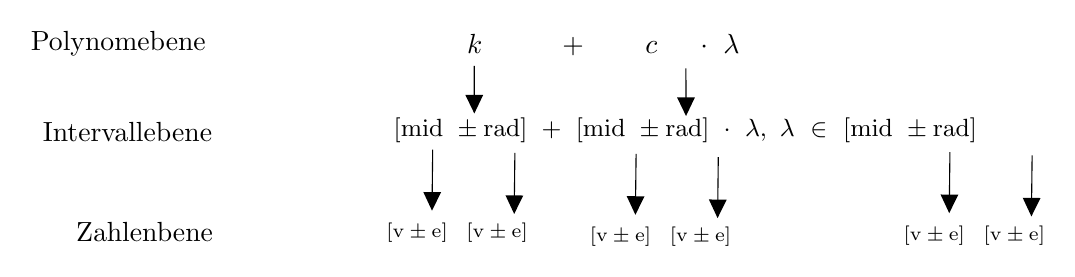
\begin{tikzpicture}[x=0.75pt,y=0.75pt,yscale=-1,xscale=1]
%uncomment if require: \path (0,300); %set diagram left start at 0, and has height of 300

%Straight Lines [id:da29898159624783616] 
\draw    (281.07,90.5) -- (280.77,116.88) ;
\draw [shift={(280.73,119.88)}, rotate = 270.65] [fill={rgb, 255:red, 0; green, 0; blue, 0 }  ][line width=0.08]  [draw opacity=0] (8.93,-4.29) -- (0,0) -- (8.93,4.29) -- cycle    ;
%Straight Lines [id:da1335093356184387] 
\draw    (320.67,92.1) -- (320.37,118.48) ;
\draw [shift={(320.33,121.48)}, rotate = 270.65] [fill={rgb, 255:red, 0; green, 0; blue, 0 }  ][line width=0.08]  [draw opacity=0] (8.93,-4.29) -- (0,0) -- (8.93,4.29) -- cycle    ;
%Straight Lines [id:da1340726243132735] 
\draw    (379.07,92.5) -- (378.77,118.88) ;
\draw [shift={(378.73,121.88)}, rotate = 270.65] [fill={rgb, 255:red, 0; green, 0; blue, 0 }  ][line width=0.08]  [draw opacity=0] (8.93,-4.29) -- (0,0) -- (8.93,4.29) -- cycle    ;
%Straight Lines [id:da9182990047680641] 
\draw    (418.67,94.1) -- (418.37,120.48) ;
\draw [shift={(418.33,123.48)}, rotate = 270.65] [fill={rgb, 255:red, 0; green, 0; blue, 0 }  ][line width=0.08]  [draw opacity=0] (8.93,-4.29) -- (0,0) -- (8.93,4.29) -- cycle    ;
%Straight Lines [id:da04610901450657834] 
\draw    (530.27,91.7) -- (529.97,118.08) ;
\draw [shift={(529.93,121.08)}, rotate = 270.65] [fill={rgb, 255:red, 0; green, 0; blue, 0 }  ][line width=0.08]  [draw opacity=0] (8.93,-4.29) -- (0,0) -- (8.93,4.29) -- cycle    ;
%Straight Lines [id:da7044032296577734] 
\draw    (569.87,93.3) -- (569.57,119.68) ;
\draw [shift={(569.53,122.68)}, rotate = 270.65] [fill={rgb, 255:red, 0; green, 0; blue, 0 }  ][line width=0.08]  [draw opacity=0] (8.93,-4.29) -- (0,0) -- (8.93,4.29) -- cycle    ;
%Straight Lines [id:da7628093943540135] 
\draw    (301.07,50.1) -- (301.12,70.08) ;
\draw [shift={(301.13,73.08)}, rotate = 269.84000000000003] [fill={rgb, 255:red, 0; green, 0; blue, 0 }  ][line width=0.08]  [draw opacity=0] (8.93,-4.29) -- (0,0) -- (8.93,4.29) -- cycle    ;
%Straight Lines [id:da9018979196177348] 
\draw    (403.07,51.3) -- (403.12,71.28) ;
\draw [shift={(403.13,74.28)}, rotate = 269.84000000000003] [fill={rgb, 255:red, 0; green, 0; blue, 0 }  ][line width=0.08]  [draw opacity=0] (8.93,-4.29) -- (0,0) -- (8.93,4.29) -- cycle    ;

% Text Node
\draw (86.2,32) node [anchor=north west][inner sep=0.75pt]   [align=left] {Polynomebene};
% Text Node
\draw (92,76) node [anchor=north west][inner sep=0.75pt]   [align=left] {Intervallebene};
% Text Node
\draw (108,124) node [anchor=north west][inner sep=0.75pt]   [align=left] {Zahlenbene};
% Text Node
\draw (296.4,33.8) node [anchor=north west][inner sep=0.75pt]    {$k\ \ \ \ \ \ \ \ +\ \ \ \ \ \  c\ \ \ \ \cdot \ \lambda $};
% Text Node
\draw (261,74) node [anchor=north west][inner sep=0.75pt]  [font=\small]  {$\left[\text{mid} \ \pm \text{rad}\right] \ +\ \left[\text{mid} \ \pm \text{rad}\right] \ \cdot \ \lambda ,\ \lambda \ \in \ \left[\text{mid} \ \pm \text{rad}\right]$};
% Text Node
\draw (257.5,124.6) node [anchor=north west][inner sep=0.75pt]  [font=\scriptsize]  {$\left[\text{v} \pm \text{e}\right] \ \ \left[\text{v} \pm \text{e}\right]$};
% Text Node
\draw (355.5,126.6) node [anchor=north west][inner sep=0.75pt]  [font=\scriptsize]  {$\left[\text{v} \pm \text{e}\right] \ \ \left[\text{v} \pm \text{e}\right]$};
% Text Node
\draw (506.7,125.8) node [anchor=north west][inner sep=0.75pt]  [font=\scriptsize]  {$\left[\text{v} \pm \text{e}\right] \ \ \left[\text{v} \pm \text{e}\right]$};


\end{tikzpicture}
  
 \caption{Ebenen der Polynomdarstellung mit REALs}
 \label{fig:levels}
 \end{center}
\end{figure}


\subsection{Präzision}
Werden zwei \verb+iRRAM-REAL+s $x$ und $y$ mit einer jeweiligen Präzision $p_x$ und $p_y$ verrechnet $z = x \circ y$, so entscheidet die Präzisions-Strategie \verb+prec_policy+, ob für für diese Operation absolute oder relative Genauigkeit verwendet wird. Zudem existiert eine globale, an die Iteration der \verb+iRRAM+ gebundene Genauigkeit \verb+actual_precision+ $p_g$ , die sich mit jeder Iteration verringert, beginnend mit dem Wert $p_{g0} = -50$. Diese Werte sind negativ und repräsentieren, die Anzahl an Bits, für die eine Zahl genau bekannt ist. Bei $z = x\circ y$ ist die Genauigkeit $p_z$ durch
$$p_z = \begin{cases}
         max(p_x, p_y, p_g) & \text{falls absolute Genauigkeit}\\
         max(p_x, p_y, max(p_x, p_y) - 50 + p_g) & \text{falls relative Genauigkeit}
        \end{cases}
$$
gegeben.
Für die Anwendung in \verb+hotm+ eignet sich die Verwendung von relativer Genauigkeit am besten, da die Manipulation der Fehlerbreite durch Cleaning große Unterschiede in der Genauigkeit zwischen Zahlen ergibt und die Skalierung zu auffwändig ist.



\section{Intervallarithmetik}
\label{sec:numint}
Arithmetik auf Taylormodellen zu betreiben bedeutet auf der untersten Ebene, mit Intervallen zu rechnen. Um diese wiederum als Zahlentyp zu verwenden, müssen die Operationen angepasst werden \cite{moore1979}.

\paragraph{Grundrechenarten}
\begin{itemize}
    \item[] $[x_1, x_2] + [y_1, y_2] = [x_1 + y_1, x_2 + y_2]$
    \item[] $[x_1, x_2] - [y_1, y_2] = [x_1 - y_2, x_2 - y_1]$
    \item[] $[x_1, x_2] \cdot [y_1, y_2] = [min(x_1 y_1, x_1 y_2, x_2 y_1, x_2 y_2), max(x_1 y_1, x_1 y_2, x_2 y_1, x_2 y_2)]$
    \item[] $[x_1, x_2] / [y_1, y_2] = [min(x_1 / y_1, x_1 / y_2, x_2 / y_1, x_2 / y_2),$\\ $max(x_1 /y_1, x_1 /y_2, x_2 /y_1, x_2 /y_2)]$
\end{itemize}
\paragraph{Potenzfunktion}\label{par:potenzfunktion}
Die Potenzfunktion unterscheidet zwischen geradem und ungeradem Exponenten.
$$[x_1, x_2]^n =
 \begin{cases}
    [x_1^n, x_2^n] & falls\ x_1 > 0\ oder\ n\ ungerade; \\
    [x_2^n, x_1^n] & falls\ x_2 < 0\ und\ n\ gerade, \\
    [0, max(x_1^n, x_2^n)] & falls\ 0\in [x_1, x_2] \ und\ n\ gerade;
 \end{cases}$$

\paragraph{Kehrwert}
Der Kehrwert eines Intervalls kann nur bestimmt werden, wenn es nicht die 0 enthält:
$$
1/[x_1, x_2] = [1/x_2, 1/x_1]
$$
Wenn $x_1 \leq 0\leq x_2$, bedeutet das, dass für ein $x\in [x_1, x_2]$, $\frac{1}{x} \geq \frac{1}{x_2}$ oder $\frac{1}{x} \leq \frac{1}{x_1}$ gelten muss und das Intervall damit unbegrenzt ist.


Die im Basisprogramm \verb+tangentspace+ vorhandene Implementierung wurde erweitert, um Punktintervalle gesondert zu behandeln und die nun auf reellen Zahlen basierenden Intervalldefinitionen zu verwenden. Dies hat zur Folge, dass die Mehrwertigkeit der Vorzeichenfunktion berücksichtigt werden muss. Tritt der Fall der Unsicherheit ein, so muss mit einer Überschätzung gerechnet werden, die in jedem Fall korrekt ist.




%% ==============================
\section{Polynommultiplikation}
%% ==============================
\label{ch:Implementierung:sec:Abschnitt1}

In einer linearen Implementierung der Taylormodelle wird bei der Multiplikation immer eines der Fehlersymbole gesweept, sodass die Länge eines Polynoms nicht über die Dimension hinausgeht und somit der Schwerpunkt bei der Intervallarithmetik liegt. Lässt man allerdings höhere Ordnungen zu, werden auch die Polynome länger und ein weiteres Problem tritt auf. Um die oben (\ref{def:order}) definierte Ordnung $\prec$ auf dem Polynom $p = p_1 \cdot p_2$ zu erhalten, müssen die $n\cdot m$ Monome ($n := \#p_1, m := \#p_2$), die bei der Multiplikation entstehen, sortiert werden. Werden diese sequentiell zu $p$ hinzugefügt bedeutet das 2 Vergleiche, dann 3, dann 4, und so weiter, bis hin zu $nm$ Vergleichen:
$$ 2 + 3 + 4 + 5 + ... + nm = \frac{nm \cdot (nm + 1)}{2} - 1$$
So ergibt sich für die naive Multiplikation eine quadratische Laufzeit in $O$-Notation von $O(nm + (nm)^2)$
\par
Für effizientere Polynommultiplikation existieren verschiedene Algorithmen. Viele der schnellen bekannten Algorithmen basieren  auf der Schnellen-Fourier-Transformation, wobei die Polynome in Stützvektoren und wieder zurück umgewandelt werden. Da es sich bei den Koeffizienten den Monome um Intervalle mit möglicherweise unendlichen Schranken handelt, ist das Rückführen eines Stützvektors nicht immer ohne Weiteres möglich. \par
Ein weiterer Ansatz besteht darin, die Anzahl der benötigten Monomvergleiche zu reduzieren, wenn die Monome einsortiert werden müssen. Betrachtet man die Summe dreier Polynome $p_1 + p_2 + p_3$ mit $\#p_1 >> \#p_2 = \#p_3 = 1$, benötigt das Aufsummieren von links nach rechts $2\#p_1 + 1$ Vergleiche, da mit dem oben verwendeten Additionsverfahren zweifach in $p_1$ eingefügt wird. Summiert man jedoch von rechts nach links so werden lediglich $\#p_1 + 2$ Vergleiche benötigt. Nach dieser Idee kann die Anzahl der Monomvergleiche reduziert werden, indem zunächst Polynome gleicher Länge miteinander addiert werden. Mit Geobuckets, von Yan (\cite{geobuckets}) eingeführt und Monagan und Pearce (\cite{geobucketsmulti}) für die Multiplikation angepasst, werden die Zwischenergebnisse der Polynommultiplikation in geometrisch wachsenden 'Buckets' gespeichert. Hat ein Bucket seine Kapazität erreicht, wird das Polynom zum nächst größeren Bucket hinzuaddiert. Der Unterschied zum Originalalgorithmus besteht darin, dass die Größe der hinzukommenden Polynome bereits bekannt ist und die Bucketkapazität dementsprechend angepasst werden kann. Algorithmus \ref{algo:mult} zeigt die in \verb+hotm+ implementierte Version der Geobucketmultiplikation. Durch den Teile und Herrsche Ansatz, kann die Multiplikation mit Geobuckets in $O(nm \log nm)$ durchgeführt werden.  \par


Wird wie in \cite{geobuckets} eine Ordnung $\succ$ auf den Monomen definiert, können die Polynome sortiert werden.
\begin{itemize}
    \label{def:order}
    \item $\lambda_1 \succ \lambda_2 \succ...\succ \lambda_k $
    \item $\lambda_n^i \lambda_m^j \succ \lambda_n^{i'} \lambda_m^{j'} $ für $n > m$, falls
    \begin{itemize}
        \item[] $ i > i'$, oder
        \item[] $ i = i'$ und $ j > j'$
    \end{itemize}
\end{itemize}
Diese Ordnung ist partiell, da gleiche Monome, beziehungsweise Monome mit gleichen Fehlersymbolen nicht vergleichbar sind. Tritt dieser Fall während der Addition zweier Polynome auf, bedeutet das, dass die Koeffizienten beider Monome addiert werden und das so entstandene Monom in das Polynom aufgenommen wird.
Haben die verglichenen Monome die selbe Anzahl an Variablen, entscheidet die Größe des Exponenten des Fehlersymbols mit dem kleinsten Index. Algorithmus \ref{algo:maxes} implementiert den Vergleich zweier Monome, beziehungsweise derer Variablen.

\begin{figure}[ht]
    \centering
    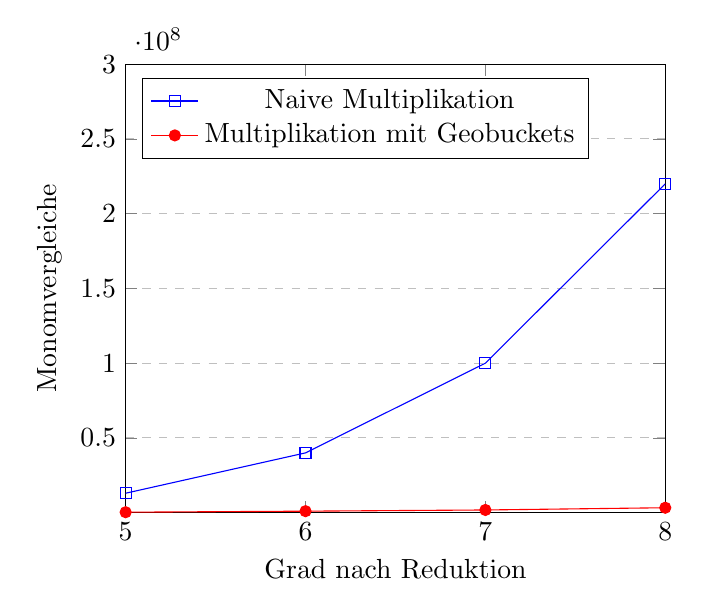
\begin{tikzpicture}
    \begin{axis}[
        xlabel={Grad nach Reduktion},
        ylabel={Monomvergleiche},
        xmin=5, xmax=8,
        ymin=100000, ymax=300000000,
        xtick={5,6,7,8},
        legend pos=north west,
        ymajorgrids=true,
        grid style=dashed,
    ]
    \addplot[
        color=blue,
        mark=square
        ]
        coordinates {
        (5, 13000000)(6, 40000000 )(7, 100000000)(8, 220000000)
        };
        \addlegendentry{Naive Multiplikation}
        
    \addplot[
        color=red,
        mark=*
        ]
        coordinates {
        (5, 300000)(6, 1000000 )(7, 1800000)(8, 3300000)
        };
        \addlegendentry{Multiplikation mit Geobuckets}
    
    \end{axis}
    \end{tikzpicture}
    \caption{Naive Multiplikation gegen Multiplikation mit Geobuckets}
    \label{fig:my_label}
\end{figure}



\newpage
%% ==============================
\section{Taylormodelle}
Taylormodelle bestehen in \verb+hotm+ aus einer List von nach der Ordnunng $\succ$ (siehe \ref{def:order}) sortierten Monomen. Für die Supportintervalle der Fehlersymbole wird eine statische Liste (\verb+static std::list+), für die Grenzwerte der Housekeeping-Methoden und den Index neuer Fehlersymbole jeweils statische Variablen angelegt.
\subsection{Housekeeping-Methoden}
Die Housekeeping-Methoden Splitting und Sweeping werden in \cite{DBLP:conf/macis/BrausseKM15} beschrieben und dienen der Kontrolle der Intervallkoeffizieten und deren Wachstum. Wann die Methoden angewandt werden, wird durch die manuell justierbaren Parameter \verb+MACRO_THRESHOLD+ für Splitting und \verb+MICRO_THRESHOLD+ für Cleaning festgelegt. Da für diese beiden Methoden Vergleiche reeller Zahlen nötig sind, um das Überschreiten eines Grenzwertes zu bestimmnen, werden die Zahlen mit Funktionen der \verb+iRRAM+ in rationale Approximationen zerlegt.

\paragraph{Cleaning}
Wie oben beschrieben, ergibt die Verwendung der \verb+iRRAM-REAL+s als Intervallgrenzen zweistufige Intervalle mit der Zahlen- und Intervallebene (siehe Abbildung \ref{fig:levels}). Mit fortlaufenden Rechnungen wächst die Breite der Intervalle auf Zahlenebene kontinuierlich und kann ohne weitere Methoden nur durch ein Erhöhen der verwendeten Präzision wieder verringer werden, beziehungsweise durch eine Iteration der \verb+iRRAM+. \textit{Cleaning} verlagert den Rechenfehler der Zahlenebene auf die Intervallebene und macht ihn damit auch für andere Housekeeping-Methoden sichtbar. Das Intervall $I=[m \pm r]$ mit $m=[c_m \pm \varepsilon_m]$ und $r = [c_r \pm \varepsilon_r]$ wird um $\varepsilon_m$ und $\varepsilon_r$ vergrößert, sodass das $I$ zwar wächst, jedoch dessen Endpunkte exakt sind:
\begin{align*}[[c_m \pm \varepsilon_m] \pm [c_r \pm \varepsilon_r]] &\rightsquigarrow [[c_m \pm 0] \pm [c_r + \varepsilon_m +\varepsilon_r  \pm 0]] \\
&= [\underbrace{c_m'}_{c_m + \varepsilon_m +\varepsilon_r} \pm c_r ]\end{align*}
    
    

\paragraph{Splitting}
Durch Cleaning, Sweeping oder eine Initialisierung der Taylormodelle mit einer gewissen Breite wachsen die Radii der Koeffizienten im Laufe einer Berechnung auch auf Intervallebene. Um die Überschätzung, die durch Intervallarithmetik entsteht zu kontrollieren, kann durch \textit{Splitting} ein Monom in zwei Monome mit Punktintervallen als Koeffizienten und einem neuen Fehlersymbol aufgeteilt werden:
\begin{align*}
[\tilde{c}_n \pm \varepsilon_n]\ \rightarrow [\tilde{c}_n \pm 0] + [\varepsilon_n \pm 0]\cdot  \lambda_n \hspace{0.5cm}, \lambda_n \in [0 \pm 1]
\end{align*}
Dadurch erhöht sich der Grad des Polynoms, jedoch verringert sich die Überschätzung durch Intervallarithmetik. Eine Alternative das Splitting zu realisieren ist, den Fehler statt wie in \cite{DBLP:conf/macis/BrausseKM15} im Koeffizienten des neuen Monoms, im neuen Fehlersymbol zu kodieren:
\begin{align*}
 [\tilde{c}_n \pm \varepsilon_n]\ \rightsquigarrow [\tilde{c}_n \pm 0] + [1 \pm 0]\cdot  \lambda_n \hspace{0.5cm}, \lambda_n \in [0 \pm \varepsilon_n]
\end{align*}
Dies hat den Vorteil, dass die Größe der Fehlersymbole beim Sweeping berücksichtigt werden kann.

\paragraph{Sweeping}
Cleaning und Splitting sorgen dafür, dass die Intervallbreite der Koeffizienten klein bleibt, jedoch erhöht sich der Grad der Polynome, was zum Beispiel bei der Multiplikation von Taylormodellen zu Ineffizienz durch die exponentiell wachsende Anzahl an Monomen führt. Um diesem Effekt entgegenzuwirken, kann mit \textit{Sweeping} ein Fehlersymbol durch sein Supportintervall ersetzt werden:
\begin{align*}
 c_n \lambda_i^k \rightsquigarrow c_n s_i \lambda_i^{k-1}
\end{align*}
Hierbei ist zu beachten, dass das $n$-fache Sweepen eines Fehlersymbols, welches die 0 enthält, mit $n$ gerade eine geringere Breite in den Koeffizienten einführt, als $n$ ungerade (siehe oben \ref{par:potenzfunktion}). Daraus ergeben sich zwei Sweeping-\textit{Strategien}.

\subparagraph{square\_only}
Die Sweeping-Strategie \verb+square_only+ beschränkt das Sweeping auf gerade Potenzen. So wird die angestrebte Reduktion des Grades eines Monoms nur erreicht, wenn alle Variablen einen geraden Exponenten haben.


\subparagraph{square\_first}
Mit \verb+square_first+ wird der angestrebte Grad erreicht, indem zunächst möglichst viele Fehlersymbole gerade gesweept werden. Falls dadurch jedoch nicht die gesamte Reduktion möglich ist, wird der Rest ungerade gesweept.

Der Aufruf der Methode erhält in \verb+hotm+ drei Parameter; das zu reduziere Taylormodell, den Grad, auf das Taylormodell durch Sweeping reduziert werden soll und die Strategie:

 \begin{lstlisting}[language=C++, caption=Beispielaufruf der Sweeping-Routine,captionpos=b,xleftmargin=15pt]
tmsimple x;
x = sweep_to(x, 2, SQUARE_ONLY);
\end{lstlisting}



\subsection{Darstellung der Taylormodelle}
Die grafischen Darstellungen der Taylormodelle in dieser Arbeit wurden mit \verb+gnuplot+ \cite{gnuplot} erstellt und zeigen je eine Übermenge des tatsächlichen Taylormodells. Eine Darstellung eines Taylormodells entsteht, indem für jedes der $k$ Fehlersymbol aus $\lambda=(\lambda_1, \dots, \lambda_k)$ ein Wert festgelegt und dann das Taylormodell evaluiert wird. Um eine Übermenge zu zeichnen muss der gesamte Wertebereich eines jeden Fehlersymbols abgedeckt werden. In \verb+hotm+ geschieht das, indem für eine gegebene \textit{Auflösung} $a \in \mathbb{N}$ die Supportintervalle $S=(s_1, \cdots s_k)$ in jeweils $a$ Intervalle geteilt und für jede Kombination mit eingesetzten Werten ein von den anderen unabhängiges Rechteck gezeichnet wird. So ergeben sich für Taylormodelle mit $k$ Variablen $a^k$ Rechtecke. Eine solche Darstellung wird in \cite{DBLP:conf/macis/BrausseKM15} als $image(T) \subseteq \mathbb{R}^d$ definiert. Die hier verwendete Darstellung wird um die verwendete Auflösung erweitert: $image_{acc}(T,a)$.

\Abbildungps{tbh}{.9}{img/accuracy.pdf}{fig:acc}{H\e non-Abbildung: Abbildung mit verschiedenen Auflösungen}{Jede Zeile zeigt eine einfache Abbildung der Rechtecke durch die H\e non-Abbildung mit $a=1.4$ und $b=0.3$ mit verschiedenen Auflösungen für die Darstellung. (a): 4 Rechtecke; (b): 100 Rechtecke, (c): 10000 Rechtecke. Das Tetragon stellt die Fangzone für die verwendeten Parameter dar. }

Seien $T_1$ und $T_2$ Taylormodelle mit $k=2$ Variablen, die eine zweidimensionale Fläche aufspannen, bei denen die initialen Fehlersymbole erhalten bleiben und keine neuen Fehlersymbole eigeführt werden, so kann durch die Abhängigkeitsinformation der Fehlersymbole Ursprung und Abbild der einzelnen Regionen dieser Fläche farblich induziert werden. Abbildung \ref{fig:acc} zeigt eine Iteration der H\e non-Abbildung eines Rechtecks mit verschiedenen Auflösungen. Es ist gut zu erkennen, dass die gröbere Auflösungen, die feinere überdeckt und $image_{acc}(T_1,100)\times image_{acc}(T_2,100) \subseteq image_{acc}(T_1,10)\times image_{acc}(T_2,10) \subseteq image_{acc}(T_1,2)\times image_{acc}(T_2,2) $ gilt. Durch die Einfärbung der Rechtecke können verschiedene Effekte beobachtet werden:
\begin{enumerate}
 \item Die Rechtecke überlagern sich im Abbild, obwohl sie sich im Ursprung nicht überschneiden und die H\e non-Abbildung an sich eindeutig invertierbar ist. Grund hierfür ist die entstehende Überschätzung durch Intervallarithmetik, die besonders bei Multiplikation, beziehungsweise Quadrierung der Intervalle zum Tragen kommt.
 \item Das in den Grafiken eingezeichnete Tetragon stellt die Fangzone $R$ für die hier verwendeten Parameter $a=1.4$ und $b=0.3$ dar. Mit Hilfe der Einfärbung ist erkennbar, wie Regionen außerhalb von $R$ wiederum außerhalb abgebildet werden, während innerhalb liegende diese nach der Abbildung nicht verlassen.
\end{enumerate}










%%% Local Variables: 
%%% mode: latex
%%% TeX-master: "thesis"
%%% End: 
    % Implementierung
%% eval.tex
%% $Id: eval.tex 61 2012-05-03 13:58:03Z bless $

\chapter{Evaluation}
\label{ch:Evaluierung}
%% ==============================
Mit verschiedenen Sweepingstrategien, Zahlentypen, Definitionsmöglichkeiten der Taylormodelle, initialer Ungenauigkeit, Genauigkeitsmodell (absolute oder relative Genauigkeit) und weiteren Einstellungsmöglichkeiten, ergibt sich ein sehr großer Suchraum zum Finden der optimalen Konfiguration für nichtlineare Taylormodelle. Allerdings ermöglichen sich dadurch sehr feingranulare Vergleiche, um herauszufinden, ob eine Implementierung nichtlinearer Taylormodelle in der Praxis schneller oder genauer als eine lineare sein kann. In diesem Kapitel werden Ergebnisse einige dieser Optionen betrachtet und versucht, die beobachteten Effekte zu erklären.

\section{Messungenauigkeiten}
\begin{align}
    x_0 &= [0 \pm 0] + [1 \pm 0] \cdot \lambda & \lambda \in [0.5 \pm \varepsilon] \label{tm1} \\ 
    x_0 &= [0.5 \pm 0] + [1 \pm 0] \cdot \lambda & \lambda \in [0 \pm \varepsilon] \label{tm2} \\
    x_0 &= [0.5 \pm 0] + [\varepsilon \pm 0] \cdot \lambda & \lambda \in [0 \pm 1] \label{tm3} \\
    x_0 &= [0 \pm 0] + [0.5 \pm \varepsilon] \cdot \lambda & \lambda \in [1 \pm 0] \label{tm4} \\
    x_0 &= [0.5 \pm 0] + [0 \pm \varepsilon] \cdot \lambda & \lambda \in [1 \pm 0] \label{tm5} \\
    x_0 &= [0.5 \pm \varepsilon] \label{tm6}
\end{align}


% 
\begin{figure}[ht]
    \centering
    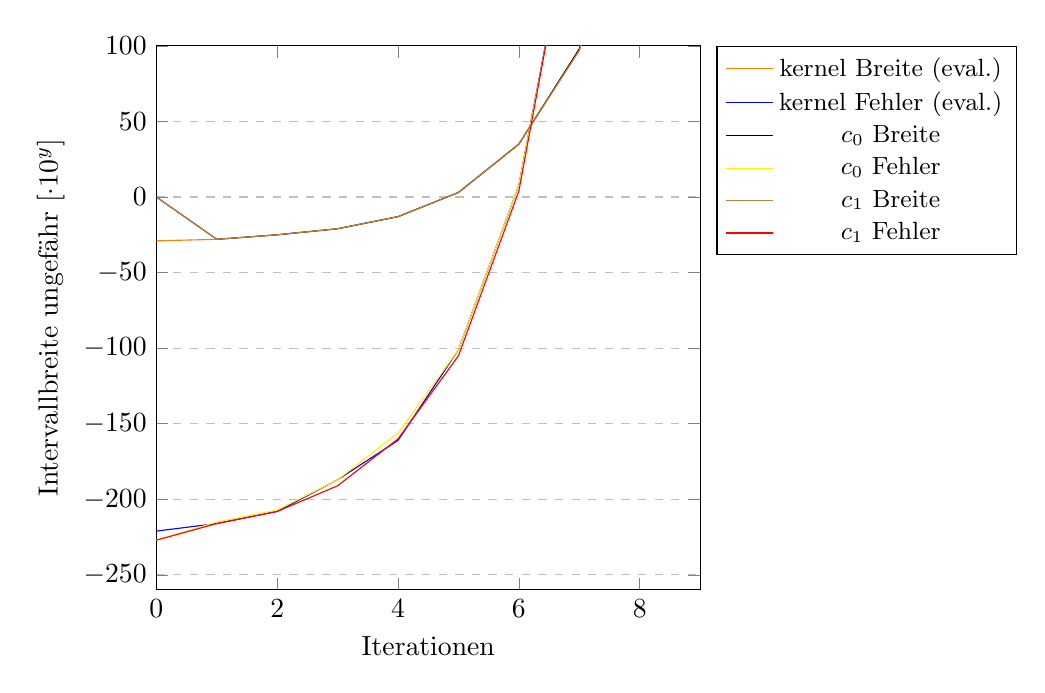
\begin{tikzpicture}
    \begin{axis}[
        width=0.7\textwidth,
        height=0.7\textwidth,
        xlabel={Iterationen},
        ylabel={Intervallbreite ungefähr $[\cdot 10^y ]$},
        legend pos=north west,
        xmin=0,xmax=9,
        ymax=100,
        ymajorgrids=true,
        grid style=dashed,
        legend pos=outer north east,
        cycle list name=color list
    ]
    
    \addplot[
        color=orange,
        ]
        coordinates {
    (0,-29)
(1,-28)
(2,-25)
(3,-21)
(4,-13)
(5,03)
(6,35)
(7,97)
(8,223)
        };
        \addlegendentry{\small{kernel Breite (eval.)}}
    
    \addplot
        coordinates {
    (0,-221)
(1,-216)
(2,-208)
(3,-187)
(4,-161)
(5,-101)
(6,8)
(7,219)
        };
        \addlegendentry{\small{kernel Fehler (eval.)}}
       
    
    \addplot
        coordinates {
    (0,0)
 (1,-28)
 (2,-25)
 (3,-21)
 (4,-13)
 (5,003)
 (6,035)
 (7,098)
 (8,223)
        };
        \addlegendentry{\small{$c_0$ Breite}}
        
    \addplot
        coordinates {
   (0,-227)
(1,-215)
(2,-207)
(3,-187)
(4,-156)
(5,-101)
(6,8)
(7,216)
(8,637)
        };
        \addlegendentry{\small{$c_0$ Fehler}}
    
        \addplot
        coordinates {
    (0,0)
 (1,-28)
 (2,-25)
 (3,-21)
 (4,-13)
 (5,+3)
 (6,+35)
 (7,+97)
 (8,+223)
        };
        \addlegendentry{\small{$c_1$ Breite}}
    
        \addplot[
        color=red,
        ]
        coordinates {
   (0,-227)
(1,-216)
(2,-208)
(3,-191)
(4,-160)
(5,-105)
(6,4)
(7,220)
        };
        \addlegendentry{\small{$c_1$ Fehler}}
    
    
    \end{axis}
    \end{tikzpicture}
    \caption{$ x_0 = [0 \pm 0] + [1 \pm 0] \cdot \lambda,\  \lambda \in [0.5 \pm \varepsilon] $}
    \label{fig:tm1}
\end{figure}
% 
\begin{figure}[ht]
    \centering
    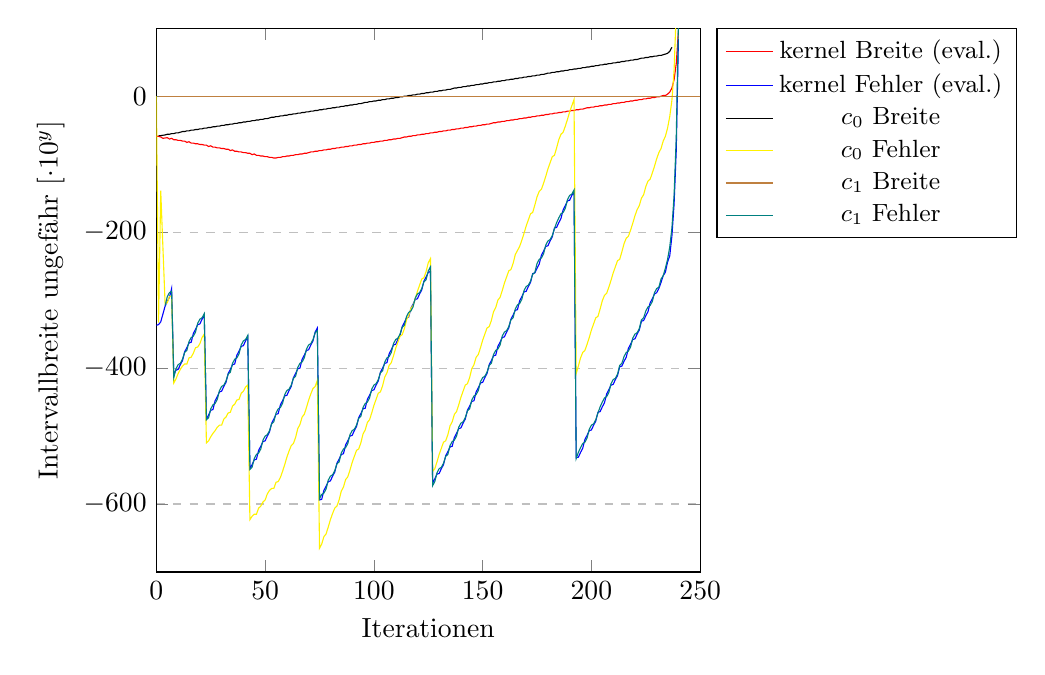
\begin{tikzpicture}
    \begin{axis}[
        width=0.7\textwidth,
        height=0.7\textwidth,
        xlabel={Iterationen},
        ylabel={Intervallbreite ungefähr $[\cdot 10^y ]$},
        legend pos=north west,
        xmin=0,xmax=250,
        ymax=100,ymin=-700,
        ymajorgrids=true,
        grid style=dashed,
        legend pos=outer north east,
        cycle list name=color list
    ]
    
    \addplot
        coordinates {
 (0,-59)
 (1,-59)
 (2,-60)
 (3,-62)
 (5,-61)
 (6,-63)
 (7,-62)
 (8,-64)
 (9,-64)
 (10,-65)
 (11,-65)
 (12,-66)
 (13,-66)
 (14,-68)
 (15,-67)
 (16,-69)
 (17,-69)
 (18,-70)
 (19,-70)
 (20,-71)
 (21,-71)
 (22,-72)
 (23,-72)
 (24,-74)
 (25,-73)
 (26,-75)
 (27,-75)
 (28,-76)
 (29,-76)
 (30,-77)
 (31,-77)
 (32,-78)
 (33,-78)
 (34,-80)
 (35,-79)
 (36,-81)
 (37,-81)
 (38,-82)
 (39,-82)
 (40,-83)
 (41,-83)
 (42,-84)
 (43,-84)
 (44,-86)
 (45,-85)
 (46,-87)
 (47,-87)
 (48,-88)
 (49,-88)
 (50,-89)
 (51,-89)
 (52,-90)
 (53,-90)
 (54,-91)
 (55,-91)
 (56,-90)
 (57,-90)
 (58,-89)
 (59,-89)
 (60,-88)
 (61,-88)
 (62,-87)
 (63,-87)
 (64,-86)
 (65,-86)
 (66,-85)
 (67,-85)
 (68,-84)
 (69,-84)
 (70,-83)
 (71,-82)
 (72,-82)
 (73,-81)
 (74,-81)
 (75,-80)
 (76,-80)
 (77,-79)
 (78,-79)
 (79,-78)
 (80,-78)
 (81,-77)
 (82,-77)
 (83,-76)
 (84,-76)
 (85,-75)
 (86,-75)
 (87,-74)
 (88,-74)
 (89,-73)
 (90,-73)
 (91,-72)
 (92,-72)
 (93,-71)
 (94,-71)
 (95,-70)
 (96,-70)
 (97,-69)
 (98,-69)
 (99,-68)
 (100,-68)
 (101,-67)
 (102,-67)
 (103,-66)
 (104,-66)
 (105,-65)
 (106,-65)
 (107,-64)
 (108,-64)
 (109,-63)
 (110,-63)
 (111,-62)
 (112,-62)
 (113,-61)
 (114,-60)
 (115,-60)
 (116,-59)
 (117,-59)
 (118,-58)
 (119,-58)
 (120,-57)
 (121,-57)
 (122,-56)
 (123,-56)
 (124,-55)
 (125,-55)
 (126,-54)
 (127,-54)
 (128,-53)
 (129,-53)
 (130,-52)
 (131,-52)
 (132,-51)
 (133,-51)
 (134,-50)
 (135,-50)
 (136,-49)
 (137,-49)
 (138,-48)
 (139,-48)
 (140,-47)
 (141,-47)
 (142,-46)
 (143,-46)
 (144,-45)
 (145,-45)
 (146,-44)
 (147,-44)
 (148,-43)
 (149,-43)
 (150,-42)
 (151,-42)
 (152,-41)
 (153,-41)
 (154,-40)
 (155,-39)
 (156,-39)
 (157,-38)
 (158,-38)
 (159,-37)
 (160,-37)
 (161,-36)
 (162,-36)
 (163,-35)
 (164,-35)
 (165,-34)
 (166,-34)
 (167,-33)
 (168,-33)
 (169,-32)
 (170,-32)
 (171,-31)
 (172,-31)
 (173,-30)
 (174,-30)
 (175,-29)
 (176,-29)
 (177,-28)
 (178,-28)
 (179,-27)
 (180,-27)
 (181,-26)
 (182,-26)
 (183,-25)
 (184,-25)
 (185,-24)
 (186,-24)
 (187,-23)
 (188,-23)
 (189,-22)
 (190,-22)
 (191,-21)
 (192,-21)
 (193,-20)
 (194,-20)
 (195,-19)
 (196,-19)
 (197,-18)
 (198,-17)
 (199,-17)
 (200,-16)
 (201,-16)
 (202,-15)
 (203,-15)
 (204,-14)
 (205,-14)
 (206,-13)
 (207,-13)
 (208,-12)
 (209,-12)
 (210,-11)
 (211,-11)
 (212,-10)
 (213,-10)
 (214,-9)
 (215,-9)
 (216,-8)
 (217,-8)
 (218,-7)
 (219,-7)
 (220,-6)
 (221,-6)
 (222,-5)
 (223,-5)
 (224,-4)
 (225,-4)
 (226,-3)
 (227,-3)
 (228,-2)
 (229,-2)
 (230,-1)
 (231,-1)
 (232,0)
 (233,1)
 (234,1)
 (235,3)
 (236,6)
 (237,12)
 (238,24)
 (239,48)
 (240,96)
        };
        \addlegendentry{\small{kernel Breite (eval.)}}
    
    \addplot
        coordinates {
(0,-337)
(1,-336)
(2,-332)
(4,-309)
(5,-302)
(6,-296)
(7,-283)
(8,-410)
(9,-403)
(10,-402)
(11,-395)
(12,-389)
(13,-376)
(14,-370)
(15,-363)
(16,-362)
(17,-349)
(18,-343)
(19,-336)
(20,-335)
(21,-328)
(22,-322)
(23,-475)
(24,-469)
(25,-462)
(26,-461)
(27,-448)
(28,-442)
(29,-435)
(30,-434)
(31,-427)
(32,-421)
(33,-408)
(34,-402)
(35,-395)
(36,-394)
(37,-381)
(38,-375)
(39,-368)
(40,-367)
(41,-360)
(42,-354)
(43,-548)
(44,-542)
(45,-535)
(46,-534)
(47,-521)
(48,-515)
(49,-508)
(50,-507)
(51,-500)
(52,-494)
(53,-481)
(54,-475)
(55,-468)
(56,-467)
(57,-454)
(58,-448)
(59,-441)
(60,-440)
(61,-433)
(62,-427)
(63,-414)
(64,-408)
(65,-401)
(66,-400)
(67,-387)
(68,-381)
(69,-374)
(70,-373)
(71,-366)
(72,-360)
(73,-347)
(74,-341)
(75,-594)
(76,-593)
(77,-580)
(78,-574)
(79,-567)
(80,-566)
(81,-559)
(82,-553)
(83,-540)
(84,-534)
(85,-527)
(86,-526)
(87,-513)
(88,-507)
(89,-500)
(90,-499)
(91,-492)
(92,-486)
(93,-473)
(94,-467)
(95,-460)
(96,-459)
(97,-446)
(98,-440)
(99,-433)
(100,-432)
(101,-425)
(102,-419)
(103,-406)
(104,-400)
(105,-393)
(106,-392)
(107,-379)
(108,-373)
(109,-366)
(110,-365)
(111,-358)
(112,-352)
(113,-339)
(114,-333)
(115,-326)
(116,-325)
(117,-312)
(118,-306)
(119,-299)
(120,-298)
(121,-291)
(122,-285)
(123,-272)
(124,-266)
(125,-259)
(126,-258)
(127,-569)
(128,-563)
(129,-556)
(130,-555)
(131,-548)
(132,-542)
(133,-529)
(134,-523)
(135,-516)
(136,-515)
(137,-502)
(138,-496)
(139,-489)
(140,-488)
(141,-481)
(142,-475)
(143,-462)
(144,-456)
(145,-449)
(146,-448)
(147,-435)
(148,-429)
(149,-422)
(150,-421)
(151,-414)
(152,-408)
(153,-395)
(154,-389)
(155,-382)
(156,-381)
(157,-368)
(158,-362)
(159,-355)
(160,-354)
(161,-347)
(162,-341)
(163,-328)
(164,-322)
(165,-315)
(166,-314)
(167,-301)
(168,-295)
(169,-288)
(170,-287)
(171,-280)
(172,-274)
(173,-261)
(174,-260)
(175,-253)
(176,-247)
(177,-234)
(178,-228)
(179,-221)
(180,-220)
(181,-213)
(182,-207)
(183,-194)
(184,-193)
(185,-186)
(186,-180)
(187,-167)
(188,-161)
(189,-154)
(190,-153)
(191,-146)
(192,-140)
(193,-532)
(194,-531)
(195,-524)
(196,-518)
(197,-505)
(198,-499)
(199,-492)
(200,-491)
(201,-484)
(202,-478)
(203,-465)
(204,-464)
(205,-457)
(206,-451)
(207,-438)
(208,-432)
(209,-425)
(210,-424)
(211,-417)
(212,-411)
(213,-398)
(214,-397)
(215,-390)
(216,-384)
(217,-371)
(218,-365)
(219,-358)
(220,-357)
(221,-350)
(222,-344)
(223,-331)
(224,-330)
(225,-323)
(226,-317)
(227,-304)
(228,-298)
(229,-291)
(230,-289)
(231,-283)
(232,-274)
(233,-264)
(234,-259)
(235,-244)
(236,-235)
(237,-206)
(238,-159)
(239,-80)
(240,84)
        };
        \addlegendentry{\small{kernel Fehler (eval.)}}
       
    
    \addplot
        coordinates {
(1,-58)
(2,-58)
(4,-57)
(5,-56)
(6,-56)
(7,-55)
(8,-55)
(9,-54)
(10,-54)
(11,-53)
(12,-52)
(13,-52)
(14,-51)
(15,-51)
(16,-50)
(17,-50)
(18,-49)
(19,-49)
(20,-48)
(21,-48)
(22,-47)
(23,-47)
(24,-46)
(25,-46)
(26,-45)
(27,-45)
(28,-44)
(29,-44)
(30,-43)
(31,-43)
(32,-42)
(33,-42)
(34,-41)
(35,-41)
(36,-40)
(37,-40)
(38,-39)
(39,-39)
(40,-38)
(41,-38)
(42,-37)
(43,-37)
(44,-36)
(45,-36)
(46,-35)
(47,-35)
(48,-34)
(49,-34)
(50,-33)
(51,-33)
(52,-32)
(53,-31)
(54,-31)
(55,-30)
(56,-30)
(57,-29)
(58,-29)
(59,-28)
(60,-28)
(61,-27)
(62,-27)
(63,-26)
(64,-26)
(65,-25)
(66,-25)
(67,-24)
(68,-24)
(69,-23)
(70,-23)
(71,-22)
(72,-22)
(73,-21)
(74,-21)
(75,-20)
(76,-20)
(77,-19)
(78,-19)
(79,-18)
(80,-18)
(81,-17)
(82,-17)
(83,-16)
(84,-16)
(85,-15)
(86,-15)
(87,-14)
(88,-14)
(89,-13)
(90,-13)
(91,-12)
(92,-12)
(93,-11)
(94,-11)
(95,-10)
(96,-9)
(97,-9)
(98,-8)
(99,-8)
(100,-7)
(101,-7)
(102,-6)
(103,-6)
(104,-5)
(105,-5)
(106,-4)
(107,-4)
(108,-3)
(109,-3)
(110,-2)
(111,-2)
(112,-1)
(113,-1)
(114,0)
(115,0)
(116,1)
(117,1)
(118,2)
(119,2)
(120,3)
(121,3)
(122,4)
(123,4)
(124,5)
(125,5)
(126,6)
(127,6)
(128,7)
(129,7)
(130,8)
(131,8)
(132,9)
(133,9)
(134,10)
(135,10)
(136,11)
(137,12)
(138,12)
(139,13)
(140,13)
(141,14)
(142,14)
(143,15)
(144,15)
(145,16)
(146,16)
(147,17)
(148,17)
(149,18)
(150,18)
(151,19)
(152,19)
(153,20)
(154,20)
(155,21)
(156,21)
(157,22)
(158,22)
(159,23)
(160,23)
(161,24)
(162,24)
(163,25)
(164,25)
(165,26)
(166,26)
(167,27)
(168,27)
(169,28)
(170,28)
(171,29)
(172,29)
(173,30)
(174,30)
(175,31)
(176,31)
(177,32)
(178,32)
(179,33)
(180,34)
(181,34)
(182,35)
(183,35)
(184,36)
(185,36)
(186,37)
(187,37)
(188,38)
(189,38)
(190,39)
(191,39)
(192,40)
(193,40)
(194,41)
(195,41)
(196,42)
(197,42)
(198,43)
(199,43)
(200,44)
(201,44)
(202,45)
(203,45)
(204,46)
(205,46)
(206,47)
(207,47)
(208,48)
(209,48)
(210,49)
(211,49)
(212,50)
(213,50)
(214,51)
(215,51)
(216,52)
(217,52)
(218,53)
(219,53)
(220,54)
(221,54)
(222,55)
(223,56)
(224,56)
(225,57)
(226,57)
(227,58)
(228,58)
(229,59)
(230,59)
(231,60)
(232,60)
(233,61)
(234,62)
(235,63)
(236,66)
(237,72)
        };
        \addlegendentry{\small{$c_0$ Breite}}
        
    \addplot
        coordinates {
 (0,0)
 (1,-333)
 (2,-139)
 (4,-305)
 (5,-304)
 (6,-295)
 (7,-294)
 (8,-422)
 (9,-416)
 (10,-408)
 (11,-402)
 (12,-397)
 (13,-394)
 (14,-394)
 (15,-385)
 (16,-384)
 (17,-378)
 (18,-370)
 (19,-369)
 (20,-364)
 (21,-355)
 (22,-350)
 (23,-510)
 (24,-507)
 (25,-501)
 (26,-496)
 (27,-492)
 (28,-487)
 (29,-484)
 (30,-484)
 (31,-475)
 (32,-472)
 (33,-466)
 (34,-465)
 (35,-456)
 (36,-453)
 (37,-447)
 (38,-446)
 (39,-437)
 (40,-434)
 (41,-428)
 (42,-425)
 (43,-623)
 (44,-618)
 (45,-615)
 (46,-615)
 (47,-606)
 (48,-603)
 (49,-597)
 (50,-594)
 (51,-585)
 (52,-580)
 (53,-577)
 (54,-577)
 (55,-568)
 (56,-567)
 (57,-561)
 (58,-552)
 (59,-542)
 (60,-531)
 (61,-522)
 (62,-514)
 (63,-511)
 (64,-502)
 (65,-489)
 (66,-483)
 (67,-472)
 (68,-468)
 (69,-458)
 (70,-447)
 (71,-438)
 (72,-430)
 (73,-427)
 (74,-418)
 (75,-665)
 (76,-659)
 (77,-648)
 (78,-644)
 (79,-634)
 (80,-623)
 (81,-614)
 (82,-606)
 (83,-603)
 (84,-594)
 (85,-581)
 (86,-575)
 (87,-564)
 (88,-560)
 (89,-550)
 (90,-539)
 (91,-530)
 (92,-521)
 (93,-519)
 (94,-510)
 (95,-497)
 (96,-491)
 (97,-480)
 (98,-476)
 (99,-466)
 (100,-455)
 (101,-446)
 (102,-437)
 (103,-435)
 (104,-426)
 (105,-413)
 (106,-407)
 (107,-396)
 (108,-392)
 (109,-382)
 (110,-371)
 (111,-362)
 (112,-353)
 (113,-351)
 (114,-342)
 (115,-329)
 (116,-323)
 (117,-312)
 (118,-308)
 (119,-298)
 (120,-287)
 (121,-278)
 (122,-269)
 (123,-267)
 (124,-258)
 (125,-245)
 (126,-239)
 (127,-552)
 (128,-548)
 (129,-538)
 (130,-527)
 (131,-518)
 (132,-509)
 (133,-507)
 (134,-498)
 (135,-485)
 (136,-479)
 (137,-468)
 (138,-464)
 (139,-454)
 (140,-443)
 (141,-434)
 (142,-425)
 (143,-423)
 (144,-414)
 (145,-401)
 (146,-395)
 (147,-384)
 (148,-380)
 (149,-370)
 (150,-359)
 (151,-350)
 (152,-341)
 (153,-339)
 (154,-330)
 (155,-317)
 (156,-311)
 (157,-300)
 (158,-296)
 (159,-286)
 (160,-275)
 (161,-266)
 (162,-257)
 (163,-255)
 (164,-246)
 (165,-233)
 (166,-227)
 (167,-221)
 (168,-212)
 (169,-202)
 (170,-191)
 (171,-182)
 (172,-173)
 (173,-171)
 (174,-160)
 (175,-148)
 (176,-140)
 (177,-137)
 (178,-128)
 (179,-118)
 (180,-107)
 (181,-98)
 (182,-89)
 (183,-87)
 (184,-76)
 (185,-64)
 (186,-56)
 (187,-53)
 (188,-44)
 (189,-34)
 (190,-23)
 (191,-14)
 (192,-5)
 (193,-408)
 (194,-397)
 (195,-385)
 (196,-377)
 (197,-374)
 (198,-365)
 (199,-355)
 (200,-344)
 (201,-335)
 (202,-326)
 (203,-324)
 (204,-313)
 (205,-301)
 (206,-293)
 (207,-290)
 (208,-281)
 (209,-271)
 (210,-260)
 (211,-251)
 (212,-242)
 (213,-240)
 (214,-229)
 (215,-217)
 (216,-209)
 (217,-206)
 (218,-197)
 (219,-187)
 (220,-176)
 (221,-167)
 (222,-161)
 (223,-150)
 (224,-145)
 (225,-133)
 (226,-125)
 (227,-122)
 (228,-113)
 (229,-103)
 (230,-92)
 (231,-83)
 (232,-77)
 (233,-66)
 (234,-59)
 (235,-47)
 (236,-30)
 (237,-6)
 (238,38)
 (239,125)
        };
        \addlegendentry{\small{$c_0$ Fehler}}
    
        \addplot
        coordinates {
 (1,0)
 (2,0)
 (4,0)
 (5,0)
 (6,0)
 (7,0)
 (8,0)
 (9,0)
 (10,0)
 (11,0)
 (12,0)
 (13,0)
 (14,0)
 (15,0)
 (16,0)
 (17,0)
 (18,0)
 (19,0)
 (20,0)
 (21,0)
 (22,0)
 (23,0)
 (24,0)
 (25,0)
 (26,0)
 (27,0)
 (28,0)
 (29,0)
 (30,0)
 (31,0)
 (32,0)
 (33,0)
 (34,0)
 (35,0)
 (36,0)
 (37,0)
 (38,0)
 (39,0)
 (40,0)
 (41,0)
 (42,0)
 (43,0)
 (44,0)
 (45,0)
 (46,0)
 (47,0)
 (48,0)
 (49,0)
 (50,0)
 (51,0)
 (52,0)
 (53,0)
 (54,0)
 (55,0)
 (56,0)
 (57,0)
 (58,0)
 (59,0)
 (60,0)
 (61,0)
 (62,0)
 (63,0)
 (64,0)
 (65,0)
 (66,0)
 (67,0)
 (68,0)
 (69,0)
 (70,0)
 (71,0)
 (72,0)
 (73,0)
 (74,0)
 (75,0)
 (76,0)
 (77,0)
 (78,0)
 (79,0)
 (80,0)
 (81,0)
 (82,0)
 (83,0)
 (84,0)
 (85,0)
 (86,0)
 (87,0)
 (88,0)
 (89,0)
 (90,0)
 (91,0)
 (92,0)
 (93,0)
 (94,0)
 (95,0)
 (96,0)
 (97,0)
 (98,0)
 (99,0)
 (100,0)
 (101,0)
 (102,0)
 (103,0)
 (104,0)
 (105,0)
 (106,0)
 (107,0)
 (108,0)
 (109,0)
 (110,0)
 (111,0)
 (112,0)
 (113,0)
 (114,0)
 (115,0)
 (116,0)
 (117,0)
 (118,0)
 (119,0)
 (120,0)
 (121,0)
 (122,0)
 (123,0)
 (124,0)
 (125,0)
 (126,0)
 (127,0)
 (128,0)
 (129,0)
 (130,0)
 (131,0)
 (132,0)
 (133,0)
 (134,0)
 (135,0)
 (136,0)
 (137,0)
 (138,0)
 (139,0)
 (140,0)
 (141,0)
 (142,0)
 (143,0)
 (144,0)
 (145,0)
 (146,0)
 (147,0)
 (148,0)
 (149,0)
 (150,0)
 (151,0)
 (152,0)
 (153,0)
 (154,0)
 (155,0)
 (156,0)
 (157,0)
 (158,0)
 (159,0)
 (160,0)
 (161,0)
 (162,0)
 (163,0)
 (164,0)
 (165,0)
 (166,0)
 (167,0)
 (168,0)
 (169,0)
 (170,0)
 (171,0)
 (172,0)
 (173,0)
 (174,0)
 (175,0)
 (176,0)
 (177,0)
 (178,0)
 (179,0)
 (180,0)
 (181,0)
 (182,0)
 (183,0)
 (184,0)
 (185,0)
 (186,0)
 (187,0)
 (188,0)
 (189,0)
 (190,0)
 (191,0)
 (192,0)
 (193,0)
 (194,0)
 (195,0)
 (196,0)
 (197,0)
 (198,0)
 (199,0)
 (200,0)
 (201,0)
 (202,0)
 (203,0)
 (204,0)
 (205,0)
 (206,0)
 (207,0)
 (208,0)
 (209,0)
 (210,0)
 (211,0)
 (212,0)
 (213,0)
 (214,0)
 (215,0)
 (216,0)
 (217,0)
 (218,0)
 (219,0)
 (220,0)
 (221,0)
 (222,0)
 (223,0)
 (224,0)
 (225,0)
 (226,0)
 (227,0)
 (228,0)
 (229,0)
 (230,0)
 (231,0)
 (232,0)
 (233,0)
 (234,0)
 (235,0)
 (236,0)
 (237,0)
 (238,0)
 (239,0)
 (240,0)
 (241,0)
 (242,0)
 (243,0)
 (244,0)
 (245,0)
 (246,0)
 (247,0)
 (248,0)
 (249,0)
 (250,0)
        };
        \addlegendentry{\small{$c_1$ Breite}}
    
        \addplot
        coordinates {
 (4,-308)
 (5,-295)
 (6,-289)
 (7,-287)
 (8,-414)
 (9,-401)
 (10,-395)
 (11,-393)
 (12,-387)
 (13,-377)
 (14,-374)
 (15,-361)
 (16,-355)
 (17,-353)
 (18,-347)
 (19,-334)
 (20,-328)
 (21,-326)
 (22,-320)
 (23,-476)
 (24,-473)
 (25,-460)
 (26,-454)
 (27,-452)
 (28,-446)
 (29,-433)
 (30,-427)
 (31,-425)
 (32,-419)
 (33,-409)
 (34,-406)
 (35,-393)
 (36,-387)
 (37,-385)
 (38,-379)
 (39,-366)
 (40,-360)
 (41,-358)
 (42,-352)
 (43,-549)
 (44,-546)
 (45,-533)
 (46,-527)
 (47,-525)
 (48,-519)
 (49,-506)
 (50,-500)
 (51,-498)
 (52,-492)
 (53,-482)
 (54,-479)
 (55,-466)
 (56,-460)
 (57,-458)
 (58,-452)
 (59,-439)
 (60,-433)
 (61,-431)
 (62,-425)
 (63,-415)
 (64,-412)
 (65,-399)
 (66,-393)
 (67,-391)
 (68,-385)
 (69,-372)
 (70,-366)
 (71,-364)
 (72,-358)
 (73,-348)
 (74,-345)
 (75,-592)
 (76,-586)
 (77,-584)
 (78,-578)
 (79,-565)
 (80,-559)
 (81,-557)
 (82,-551)
 (83,-541)
 (84,-538)
 (85,-525)
 (86,-519)
 (87,-517)
 (88,-511)
 (89,-498)
 (90,-492)
 (91,-490)
 (92,-484)
 (93,-474)
 (94,-471)
 (95,-458)
 (96,-452)
 (97,-450)
 (98,-444)
 (99,-431)
 (100,-425)
 (101,-423)
 (102,-417)
 (103,-407)
 (104,-404)
 (105,-391)
 (106,-385)
 (107,-383)
 (108,-377)
 (109,-364)
 (110,-358)
 (111,-356)
 (112,-350)
 (113,-340)
 (114,-337)
 (115,-324)
 (116,-318)
 (117,-316)
 (118,-310)
 (119,-297)
 (120,-291)
 (121,-289)
 (122,-283)
 (123,-273)
 (124,-270)
 (125,-257)
 (126,-251)
 (127,-573)
 (128,-567)
 (129,-554)
 (130,-548)
 (131,-546)
 (132,-540)
 (133,-530)
 (134,-527)
 (135,-514)
 (136,-508)
 (137,-506)
 (138,-500)
 (139,-487)
 (140,-481)
 (141,-479)
 (142,-473)
 (143,-463)
 (144,-460)
 (145,-447)
 (146,-441)
 (147,-439)
 (148,-433)
 (149,-420)
 (150,-414)
 (151,-412)
 (152,-406)
 (153,-396)
 (154,-393)
 (155,-380)
 (156,-374)
 (157,-372)
 (158,-366)
 (159,-353)
 (160,-347)
 (161,-345)
 (162,-339)
 (163,-329)
 (164,-326)
 (165,-313)
 (166,-307)
 (167,-305)
 (168,-299)
 (169,-286)
 (170,-280)
 (171,-278)
 (172,-272)
 (173,-262)
 (174,-259)
 (175,-246)
 (176,-240)
 (177,-238)
 (178,-232)
 (179,-219)
 (180,-213)
 (181,-211)
 (182,-205)
 (183,-195)
 (184,-186)
 (185,-179)
 (186,-173)
 (187,-171)
 (188,-165)
 (189,-152)
 (190,-146)
 (191,-144)
 (192,-138)
 (193,-533)
 (194,-524)
 (195,-517)
 (196,-511)
 (197,-509)
 (198,-503)
 (199,-490)
 (200,-484)
 (201,-482)
 (202,-476)
 (203,-466)
 (204,-457)
 (205,-450)
 (206,-444)
 (207,-442)
 (208,-436)
 (209,-423)
 (210,-417)
 (211,-415)
 (212,-409)
 (213,-396)
 (214,-393)
 (215,-383)
 (216,-377)
 (217,-375)
 (218,-369)
 (219,-356)
 (220,-350)
 (221,-348)
 (222,-342)
 (223,-329)
 (224,-326)
 (225,-316)
 (226,-310)
 (227,-308)
 (228,-302)
 (229,-289)
 (230,-283)
 (231,-281)
 (232,-269)
 (233,-264)
 (234,-253)
 (235,-240)
 (236,-222)
 (237,-194)
 (238,-146)
 (239,-60)
 (240,108)
 (241,436)
        };
        \addlegendentry{\small{$c_1$ Fehler}}
    
    
    \end{axis}
    \end{tikzpicture}
    \caption{$x_0 = [0.5 \pm 0] + [1 \pm 0] \cdot \lambda,\  \lambda \in [0 \pm \varepsilon]$}
    \label{fig:tm2}
\end{figure}
% 
\begin{figure}[ht]
    \centering
    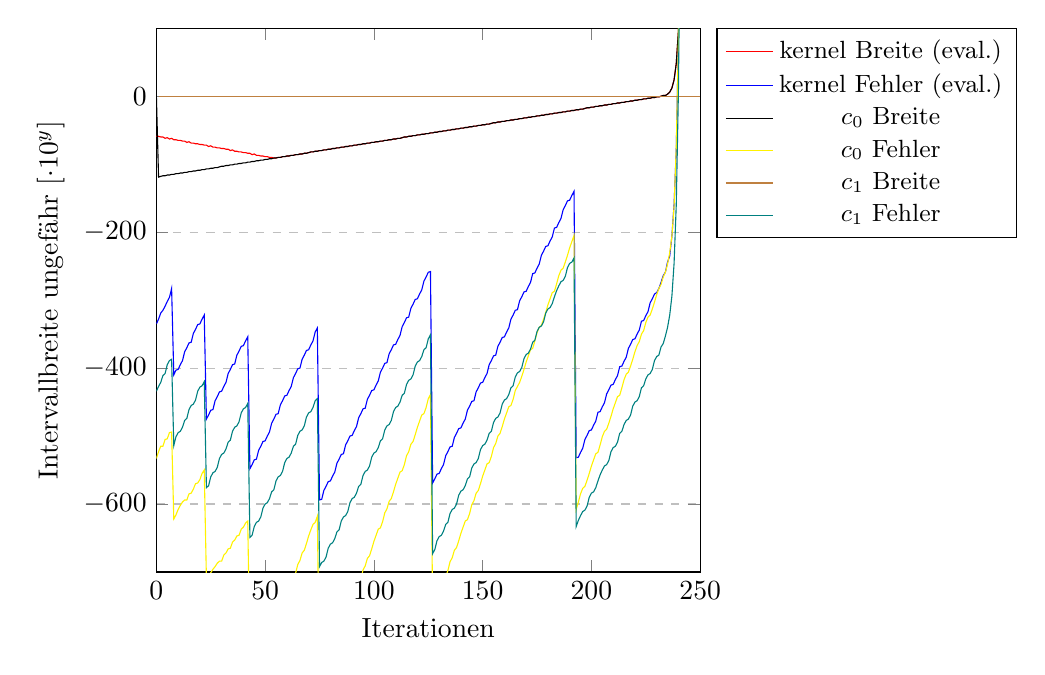
\begin{tikzpicture}
    \begin{axis}[
        width=0.7\textwidth,
        height=0.7\textwidth,
        xlabel={Iterationen},
        ylabel={Intervallbreite ungefähr $[\cdot 10^y ]$},
        legend pos=north west,
        xmin=0,xmax=250,
        ymax=100,ymin=-700,
        ymajorgrids=true,
        grid style=dashed,
        legend pos=outer north east,
        cycle list name=color list
    ]
    
    \addplot
        coordinates {
  (0,-59)
 (1,-59)
 (2,-60)
 (3,-60)
 (4,-62)
 (5,-61)
 (6,-63)
 (7,-62)
 (8,-64)
 (9,-64)
 (10,-65)
 (11,-65)
 (12,-66)
 (13,-66)
 (14,-68)
 (15,-67)
 (16,-69)
 (17,-69)
 (18,-70)
 (19,-70)
 (20,-71)
 (21,-71)
 (22,-72)
 (23,-72)
 (24,-74)
 (25,-73)
 (26,-75)
 (27,-75)
 (28,-76)
 (29,-76)
 (30,-77)
 (31,-77)
 (32,-78)
 (33,-78)
 (34,-80)
 (35,-79)
 (36,-81)
 (37,-81)
 (38,-82)
 (39,-82)
 (40,-83)
 (41,-83)
 (42,-84)
 (43,-84)
 (44,-86)
 (45,-85)
 (46,-87)
 (47,-87)
 (48,-88)
 (49,-88)
 (50,-89)
 (51,-89)
 (52,-90)
 (53,-90)
 (54,-91)
 (55,-91)
 (56,-90)
 (57,-90)
 (58,-89)
 (59,-89)
 (60,-88)
 (61,-88)
 (62,-87)
 (63,-87)
 (64,-86)
 (65,-86)
 (66,-85)
 (67,-85)
 (68,-84)
 (69,-84)
 (70,-83)
 (71,-82)
 (72,-82)
 (73,-81)
 (74,-81)
 (75,-80)
 (76,-80)
 (77,-79)
 (78,-79)
 (79,-78)
 (80,-78)
 (81,-77)
 (82,-77)
 (83,-76)
 (84,-76)
 (85,-75)
 (86,-75)
 (87,-74)
 (88,-74)
 (89,-73)
 (90,-73)
 (91,-72)
 (92,-72)
 (93,-71)
 (94,-71)
 (95,-70)
 (96,-70)
 (97,-69)
 (98,-69)
 (99,-68)
 (100,-68)
 (101,-67)
 (102,-67)
 (103,-66)
 (104,-66)
 (105,-65)
 (106,-65)
 (107,-64)
 (108,-64)
 (109,-63)
 (110,-63)
 (111,-62)
 (112,-62)
 (113,-61)
 (114,-60)
 (115,-60)
 (116,-59)
 (117,-59)
 (118,-58)
 (119,-58)
 (120,-57)
 (121,-57)
 (122,-56)
 (123,-56)
 (124,-55)
 (125,-55)
 (126,-54)
 (127,-54)
 (128,-53)
 (129,-53)
 (130,-52)
 (131,-52)
 (132,-51)
 (133,-51)
 (134,-50)
 (135,-50)
 (136,-49)
 (137,-49)
 (138,-48)
 (139,-48)
 (140,-47)
 (141,-47)
 (142,-46)
 (143,-46)
 (144,-45)
 (145,-45)
 (146,-44)
 (147,-44)
 (148,-43)
 (149,-43)
 (150,-42)
 (151,-42)
 (152,-41)
 (153,-41)
 (154,-40)
 (155,-39)
 (156,-39)
 (157,-38)
 (158,-38)
 (159,-37)
 (160,-37)
 (161,-36)
 (162,-36)
 (163,-35)
 (164,-35)
 (165,-34)
 (166,-34)
 (167,-33)
 (168,-33)
 (169,-32)
 (170,-32)
 (171,-31)
 (172,-31)
 (173,-30)
 (174,-30)
 (175,-29)
 (176,-29)
 (177,-28)
 (178,-28)
 (179,-27)
 (180,-27)
 (181,-26)
 (182,-26)
 (183,-25)
 (184,-25)
 (185,-24)
 (186,-24)
 (187,-23)
 (188,-23)
 (189,-22)
 (190,-22)
 (191,-21)
 (192,-21)
 (193,-20)
 (194,-20)
 (195,-19)
 (196,-19)
 (197,-18)
 (198,-17)
 (199,-17)
 (200,-16)
 (201,-16)
 (202,-15)
 (203,-15)
 (204,-14)
 (205,-14)
 (206,-13)
 (207,-13)
 (208,-12)
 (209,-12)
 (210,-11)
 (211,-11)
 (212,-10)
 (213,-10)
 (214,-9)
 (215,-9)
 (216,-8)
 (217,-8)
 (218,-7)
 (219,-7)
 (220,-6)
 (221,-6)
 (222,-5)
 (223,-5)
 (224,-4)
 (225,-4)
 (226,-3)
 (227,-3)
 (228,-2)
 (229,-2)
 (230,-1)
 (231,-1)
 (232,0)
 (233,01)
 (234,01)
 (235,03)
 (236,06)
 (237,012)
 (238,024)
 (239,048)
 (240,096)
 (241,0192)
        };
        \addlegendentry{\small{kernel Breite (eval.)}}
    
    \addplot
        coordinates {
 (0,-335)
 (1,-328)
 (2,-319)
 (3,-315)
 (4,-309)
 (5,-302)
 (6,-296)
 (7,-283)
 (8,-410)
 (9,-403)
 (10,-402)
 (11,-395)
 (12,-389)
 (13,-376)
 (14,-370)
 (15,-363)
 (16,-362)
 (17,-349)
 (18,-343)
 (19,-336)
 (20,-335)
 (21,-328)
 (22,-322)
 (23,-475)
 (24,-469)
 (25,-462)
 (26,-461)
 (27,-448)
 (28,-442)
 (29,-435)
 (30,-434)
 (31,-427)
 (32,-421)
 (33,-408)
 (34,-402)
 (35,-395)
 (36,-394)
 (37,-381)
 (38,-375)
 (39,-368)
 (40,-367)
 (41,-360)
 (42,-354)
 (43,-548)
 (44,-542)
 (45,-535)
 (46,-534)
 (47,-521)
 (48,-515)
 (49,-508)
 (50,-507)
 (51,-500)
 (52,-494)
 (53,-481)
 (54,-475)
 (55,-468)
 (56,-467)
 (57,-454)
 (58,-448)
 (59,-441)
 (60,-440)
 (61,-433)
 (62,-427)
 (63,-414)
 (64,-408)
 (65,-401)
 (66,-400)
 (67,-387)
 (68,-381)
 (69,-374)
 (70,-373)
 (71,-366)
 (72,-360)
 (73,-347)
 (74,-341)
 (75,-594)
 (76,-593)
 (77,-580)
 (78,-574)
 (79,-567)
 (80,-566)
 (81,-559)
 (82,-553)
 (83,-540)
 (84,-534)
 (85,-527)
 (86,-526)
 (87,-513)
 (88,-507)
 (89,-500)
 (90,-499)
 (91,-492)
 (92,-486)
 (93,-473)
 (94,-467)
 (95,-460)
 (96,-459)
 (97,-446)
 (98,-440)
 (99,-433)
 (100,-432)
 (101,-425)
 (102,-419)
 (103,-406)
 (104,-400)
 (105,-393)
 (106,-392)
 (107,-379)
 (108,-373)
 (109,-366)
 (110,-365)
 (111,-358)
 (112,-352)
 (113,-339)
 (114,-333)
 (115,-326)
 (116,-325)
 (117,-312)
 (118,-306)
 (119,-299)
 (120,-298)
 (121,-291)
 (122,-285)
 (123,-272)
 (124,-266)
 (125,-259)
 (126,-258)
 (127,-569)
 (128,-563)
 (129,-556)
 (130,-555)
 (131,-548)
 (132,-542)
 (133,-529)
 (134,-523)
 (135,-516)
 (136,-515)
 (137,-502)
 (138,-496)
 (139,-489)
 (140,-488)
 (141,-481)
 (142,-475)
 (143,-462)
 (144,-456)
 (145,-449)
 (146,-448)
 (147,-435)
 (148,-429)
 (149,-422)
 (150,-421)
 (151,-414)
 (152,-408)
 (153,-395)
 (154,-389)
 (155,-382)
 (156,-381)
 (157,-368)
 (158,-362)
 (159,-355)
 (160,-354)
 (161,-347)
 (162,-341)
 (163,-328)
 (164,-322)
 (165,-315)
 (166,-314)
 (167,-301)
 (168,-295)
 (169,-288)
 (170,-287)
 (171,-280)
 (172,-274)
 (173,-261)
 (174,-260)
 (175,-253)
 (176,-247)
 (177,-234)
 (178,-228)
 (179,-221)
 (180,-220)
 (181,-213)
 (182,-207)
 (183,-194)
 (184,-193)
 (185,-186)
 (186,-180)
 (187,-167)
 (188,-161)
 (189,-154)
 (190,-153)
 (191,-146)
 (192,-140)
 (193,-532)
 (194,-531)
 (195,-524)
 (196,-518)
 (197,-505)
 (198,-499)
 (199,-492)
 (200,-491)
 (201,-484)
 (202,-478)
 (203,-465)
 (204,-464)
 (205,-457)
 (206,-451)
 (207,-438)
 (208,-432)
 (209,-425)
 (210,-424)
 (211,-417)
 (212,-411)
 (213,-398)
 (214,-397)
 (215,-390)
 (216,-384)
 (217,-371)
 (218,-365)
 (219,-358)
 (220,-357)
 (221,-350)
 (222,-344)
 (223,-331)
 (224,-330)
 (225,-323)
 (226,-317)
 (227,-304)
 (228,-298)
 (229,-291)
 (230,-289)
 (231,-283)
 (232,-274)
 (233,-264)
 (234,-259)
 (235,-244)
 (236,-235)
 (237,-206)
 (238,-159)
 (239,-80)
 (240,84)
        };
        \addlegendentry{\small{kernel Fehler (eval.)}}
       
    
    \addplot
        coordinates {
(0,0)
 (1,-119)
 (2,-118)
 (3,-117)
 (4,-117)
 (5,-116)
 (6,-116)
 (7,-115)
 (8,-115)
 (9,-114)
 (10,-114)
 (11,-113)
 (12,-113)
 (13,-112)
 (14,-112)
 (15,-111)
 (16,-111)
 (17,-110)
 (18,-110)
 (19,-109)
 (20,-109)
 (21,-108)
 (22,-108)
 (23,-107)
 (24,-107)
 (25,-106)
 (26,-106)
 (27,-105)
 (28,-105)
 (29,-104)
 (30,-103)
 (31,-103)
 (32,-102)
 (33,-102)
 (34,-101)
 (35,-101)
 (36,-100)
 (37,-100)
 (38,-99)
 (39,-99)
 (40,-98)
 (41,-98)
 (42,-97)
 (43,-97)
 (44,-96)
 (45,-96)
 (46,-95)
 (47,-95)
 (48,-94)
 (49,-94)
 (50,-93)
 (51,-93)
 (52,-92)
 (53,-92)
 (54,-91)
 (55,-91)
 (56,-90)
 (57,-90)
 (58,-89)
 (59,-89)
 (60,-88)
 (61,-88)
 (62,-87)
 (63,-87)
 (64,-86)
 (65,-86)
 (66,-85)
 (67,-85)
 (68,-84)
 (69,-84)
 (70,-83)
 (71,-82)
 (72,-82)
 (73,-81)
 (74,-81)
 (75,-80)
 (76,-80)
 (77,-79)
 (78,-79)
 (79,-78)
 (80,-78)
 (81,-77)
 (82,-77)
 (83,-76)
 (84,-76)
 (85,-75)
 (86,-75)
 (87,-74)
 (88,-74)
 (89,-73)
 (90,-73)
 (91,-72)
 (92,-72)
 (93,-71)
 (94,-71)
 (95,-70)
 (96,-70)
 (97,-69)
 (98,-69)
 (99,-68)
 (100,-68)
 (101,-67)
 (102,-67)
 (103,-66)
 (104,-66)
 (105,-65)
 (106,-65)
 (107,-64)
 (108,-64)
 (109,-63)
 (110,-63)
 (111,-62)
 (112,-62)
 (113,-61)
 (114,-60)
 (115,-60)
 (116,-59)
 (117,-59)
 (118,-58)
 (119,-58)
 (120,-57)
 (121,-57)
 (122,-56)
 (123,-56)
 (124,-55)
 (125,-55)
 (126,-54)
 (127,-54)
 (128,-53)
 (129,-53)
 (130,-52)
 (131,-52)
 (132,-51)
 (133,-51)
 (134,-50)
 (135,-50)
 (136,-49)
 (137,-49)
 (138,-48)
 (139,-48)
 (140,-47)
 (141,-47)
 (142,-46)
 (143,-46)
 (144,-45)
 (145,-45)
 (146,-44)
 (147,-44)
 (148,-43)
 (149,-43)
 (150,-42)
 (151,-42)
 (152,-41)
 (153,-41)
 (154,-40)
 (155,-39)
 (156,-39)
 (157,-38)
 (158,-38)
 (159,-37)
 (160,-37)
 (161,-36)
 (162,-36)
 (163,-35)
 (164,-35)
 (165,-34)
 (166,-34)
 (167,-33)
 (168,-33)
 (169,-32)
 (170,-32)
 (171,-31)
 (172,-31)
 (173,-30)
 (174,-30)
 (175,-29)
 (176,-29)
 (177,-28)
 (178,-28)
 (179,-27)
 (180,-27)
 (181,-26)
 (182,-26)
 (183,-25)
 (184,-25)
 (185,-24)
 (186,-24)
 (187,-23)
 (188,-23)
 (189,-22)
 (190,-22)
 (191,-21)
 (192,-21)
 (193,-20)
 (194,-20)
 (195,-19)
 (196,-19)
 (197,-18)
 (198,-17)
 (199,-17)
 (200,-16)
 (201,-16)
 (202,-15)
 (203,-15)
 (204,-14)
 (205,-14)
 (206,-13)
 (207,-13)
 (208,-12)
 (209,-12)
 (210,-11)
 (211,-11)
 (212,-10)
 (213,-10)
 (214,-9)
 (215,-9)
 (216,-8)
 (217,-8)
 (218,-7)
 (219,-7)
 (220,-6)
 (221,-6)
 (222,-5)
 (223,-5)
 (224,-4)
 (225,-4)
 (226,-3)
 (227,-3)
 (228,-2)
 (229,-2)
 (230,-1)
 (231,-1)
 (232,0)
 (233,01)
 (234,01)
 (235,03)
 (236,06)
 (237,012)
 (238,024)
 (239,048)
 (240,096)
 (241,0192)
        };
        \addlegendentry{\small{$c_0$ Breite}}
        
    \addplot
        coordinates {
  (0,-533)
 (1,-523)
 (2,-515)
 (3,-515)
 (4,-505)
 (5,-504)
 (6,-495)
 (7,-494)
 (8,-622)
 (9,-616)
 (10,-608)
 (11,-602)
 (12,-597)
 (13,-594)
 (14,-594)
 (15,-585)
 (16,-584)
 (17,-578)
 (18,-570)
 (19,-569)
 (20,-564)
 (21,-555)
 (22,-550)
 (23,-710)
 (24,-707)
 (25,-701)
 (26,-696)
 (27,-692)
 (28,-687)
 (29,-684)
 (30,-684)
 (31,-675)
 (32,-672)
 (33,-666)
 (34,-665)
 (35,-656)
 (36,-653)
 (37,-647)
 (38,-646)
 (39,-637)
 (40,-634)
 (41,-628)
 (42,-625)
 (43,-823)
 (44,-818)
 (45,-815)
 (46,-815)
 (47,-806)
 (48,-803)
 (49,-797)
 (50,-794)
 (51,-785)
 (52,-780)
 (53,-777)
 (54,-777)
 (55,-768)
 (56,-767)
 (57,-761)
 (58,-752)
 (59,-742)
 (60,-731)
 (61,-722)
 (62,-714)
 (63,-711)
 (64,-702)
 (65,-689)
 (66,-683)
 (67,-672)
 (68,-668)
 (69,-658)
 (70,-647)
 (71,-638)
 (72,-630)
 (73,-627)
 (74,-618)
 (75,-865)
 (76,-859)
 (77,-848)
 (78,-844)
 (79,-834)
 (80,-823)
 (81,-814)
 (82,-806)
 (83,-803)
 (84,-794)
 (85,-781)
 (86,-775)
 (87,-764)
 (88,-760)
 (89,-750)
 (90,-739)
 (91,-730)
 (92,-721)
 (93,-719)
 (94,-710)
 (95,-697)
 (96,-691)
 (97,-680)
 (98,-676)
 (99,-666)
 (100,-655)
 (101,-646)
 (102,-637)
 (103,-635)
 (104,-626)
 (105,-613)
 (106,-607)
 (107,-596)
 (108,-592)
 (109,-582)
 (110,-571)
 (111,-562)
 (112,-553)
 (113,-551)
 (114,-542)
 (115,-529)
 (116,-523)
 (117,-512)
 (118,-508)
 (119,-498)
 (120,-487)
 (121,-478)
 (122,-469)
 (123,-467)
 (124,-458)
 (125,-445)
 (126,-439)
 (127,-752)
 (128,-748)
 (129,-738)
 (130,-727)
 (131,-718)
 (132,-709)
 (133,-707)
 (134,-698)
 (135,-685)
 (136,-679)
 (137,-668)
 (138,-664)
 (139,-654)
 (140,-643)
 (141,-634)
 (142,-625)
 (143,-623)
 (144,-614)
 (145,-601)
 (146,-595)
 (147,-584)
 (148,-580)
 (149,-570)
 (150,-559)
 (151,-550)
 (152,-541)
 (153,-539)
 (154,-530)
 (155,-517)
 (156,-511)
 (157,-500)
 (158,-496)
 (159,-486)
 (160,-475)
 (161,-466)
 (162,-457)
 (163,-455)
 (164,-446)
 (165,-433)
 (166,-427)
 (167,-421)
 (168,-412)
 (169,-402)
 (170,-391)
 (171,-382)
 (172,-373)
 (173,-371)
 (174,-360)
 (175,-348)
 (176,-340)
 (177,-337)
 (178,-328)
 (179,-318)
 (180,-307)
 (181,-298)
 (182,-289)
 (183,-287)
 (184,-276)
 (185,-264)
 (186,-256)
 (187,-253)
 (188,-244)
 (189,-234)
 (190,-223)
 (191,-214)
 (192,-205)
 (193,-608)
 (194,-597)
 (195,-585)
 (196,-577)
 (197,-574)
 (198,-565)
 (199,-555)
 (200,-544)
 (201,-535)
 (202,-526)
 (203,-524)
 (204,-513)
 (205,-501)
 (206,-493)
 (207,-490)
 (208,-481)
 (209,-471)
 (210,-460)
 (211,-451)
 (212,-442)
 (213,-440)
 (214,-429)
 (215,-417)
 (216,-409)
 (217,-406)
 (218,-397)
 (219,-387)
 (220,-376)
 (221,-367)
 (222,-361)
 (223,-350)
 (224,-345)
 (225,-333)
 (226,-325)
 (227,-322)
 (228,-313)
 (229,-303)
 (230,-292)
 (231,-283)
 (232,-277)
 (233,-266)
 (234,-259)
 (235,-247)
 (236,-230)
 (237,-206)
 (238,-162)
 (239,-75)
 (240,84)
 (241,408)
        };
        \addlegendentry{\small{$c_0$ Fehler}}
    
        \addplot
        coordinates {
 (1,0)
 (2,0)
 (4,0)
 (5,0)
 (6,0)
 (7,0)
 (8,0)
 (9,0)
 (10,0)
 (11,0)
 (12,0)
 (13,0)
 (14,0)
 (15,0)
 (16,0)
 (17,0)
 (18,0)
 (19,0)
 (20,0)
 (21,0)
 (22,0)
 (23,0)
 (24,0)
 (25,0)
 (26,0)
 (27,0)
 (28,0)
 (29,0)
 (30,0)
 (31,0)
 (32,0)
 (33,0)
 (34,0)
 (35,0)
 (36,0)
 (37,0)
 (38,0)
 (39,0)
 (40,0)
 (41,0)
 (42,0)
 (43,0)
 (44,0)
 (45,0)
 (46,0)
 (47,0)
 (48,0)
 (49,0)
 (50,0)
 (51,0)
 (52,0)
 (53,0)
 (54,0)
 (55,0)
 (56,0)
 (57,0)
 (58,0)
 (59,0)
 (60,0)
 (61,0)
 (62,0)
 (63,0)
 (64,0)
 (65,0)
 (66,0)
 (67,0)
 (68,0)
 (69,0)
 (70,0)
 (71,0)
 (72,0)
 (73,0)
 (74,0)
 (75,0)
 (76,0)
 (77,0)
 (78,0)
 (79,0)
 (80,0)
 (81,0)
 (82,0)
 (83,0)
 (84,0)
 (85,0)
 (86,0)
 (87,0)
 (88,0)
 (89,0)
 (90,0)
 (91,0)
 (92,0)
 (93,0)
 (94,0)
 (95,0)
 (96,0)
 (97,0)
 (98,0)
 (99,0)
 (100,0)
 (101,0)
 (102,0)
 (103,0)
 (104,0)
 (105,0)
 (106,0)
 (107,0)
 (108,0)
 (109,0)
 (110,0)
 (111,0)
 (112,0)
 (113,0)
 (114,0)
 (115,0)
 (116,0)
 (117,0)
 (118,0)
 (119,0)
 (120,0)
 (121,0)
 (122,0)
 (123,0)
 (124,0)
 (125,0)
 (126,0)
 (127,0)
 (128,0)
 (129,0)
 (130,0)
 (131,0)
 (132,0)
 (133,0)
 (134,0)
 (135,0)
 (136,0)
 (137,0)
 (138,0)
 (139,0)
 (140,0)
 (141,0)
 (142,0)
 (143,0)
 (144,0)
 (145,0)
 (146,0)
 (147,0)
 (148,0)
 (149,0)
 (150,0)
 (151,0)
 (152,0)
 (153,0)
 (154,0)
 (155,0)
 (156,0)
 (157,0)
 (158,0)
 (159,0)
 (160,0)
 (161,0)
 (162,0)
 (163,0)
 (164,0)
 (165,0)
 (166,0)
 (167,0)
 (168,0)
 (169,0)
 (170,0)
 (171,0)
 (172,0)
 (173,0)
 (174,0)
 (175,0)
 (176,0)
 (177,0)
 (178,0)
 (179,0)
 (180,0)
 (181,0)
 (182,0)
 (183,0)
 (184,0)
 (185,0)
 (186,0)
 (187,0)
 (188,0)
 (189,0)
 (190,0)
 (191,0)
 (192,0)
 (193,0)
 (194,0)
 (195,0)
 (196,0)
 (197,0)
 (198,0)
 (199,0)
 (200,0)
 (201,0)
 (202,0)
 (203,0)
 (204,0)
 (205,0)
 (206,0)
 (207,0)
 (208,0)
 (209,0)
 (210,0)
 (211,0)
 (212,0)
 (213,0)
 (214,0)
 (215,0)
 (216,0)
 (217,0)
 (218,0)
 (219,0)
 (220,0)
 (221,0)
 (222,0)
 (223,0)
 (224,0)
 (225,0)
 (226,0)
 (227,0)
 (228,0)
 (229,0)
 (230,0)
 (231,0)
 (232,0)
 (233,0)
 (234,0)
 (235,0)
 (236,0)
 (237,0)
 (238,0)
 (239,0)
 (240,0)
 (241,0)
 (242,0)
 (243,0)
 (244,0)
 (245,0)
 (246,0)
 (247,0)
 (248,0)
 (249,0)
 (250,0)
        };
        \addlegendentry{\small{$c_1$ Breite}}
    
        \addplot
        coordinates {
  (0,-434)
 (1,-427)
 (2,-421)
 (3,-411)
 (4,-408)
 (5,-395)
 (6,-389)
 (7,-387)
 (8,-514)
 (9,-501)
 (10,-495)
 (11,-493)
 (12,-487)
 (13,-477)
 (14,-474)
 (15,-461)
 (16,-455)
 (17,-453)
 (18,-447)
 (19,-434)
 (20,-428)
 (21,-426)
 (22,-420)
 (23,-576)
 (24,-573)
 (25,-560)
 (26,-554)
 (27,-552)
 (28,-546)
 (29,-533)
 (30,-527)
 (31,-525)
 (32,-519)
 (33,-509)
 (34,-506)
 (35,-493)
 (36,-487)
 (37,-485)
 (38,-479)
 (39,-466)
 (40,-460)
 (41,-458)
 (42,-452)
 (43,-649)
 (44,-646)
 (45,-633)
 (46,-627)
 (47,-625)
 (48,-619)
 (49,-606)
 (50,-600)
 (51,-598)
 (52,-592)
 (53,-582)
 (54,-579)
 (55,-566)
 (56,-560)
 (57,-558)
 (58,-552)
 (59,-539)
 (60,-533)
 (61,-531)
 (62,-525)
 (63,-515)
 (64,-512)
 (65,-499)
 (66,-493)
 (67,-491)
 (68,-485)
 (69,-472)
 (70,-466)
 (71,-464)
 (72,-458)
 (73,-448)
 (74,-445)
 (75,-692)
 (76,-686)
 (77,-684)
 (78,-678)
 (79,-665)
 (80,-659)
 (81,-657)
 (82,-651)
 (83,-641)
 (84,-638)
 (85,-625)
 (86,-619)
 (87,-617)
 (88,-611)
 (89,-598)
 (90,-592)
 (91,-590)
 (92,-584)
 (93,-574)
 (94,-571)
 (95,-558)
 (96,-552)
 (97,-550)
 (98,-544)
 (99,-531)
 (100,-525)
 (101,-523)
 (102,-517)
 (103,-507)
 (104,-504)
 (105,-491)
 (106,-485)
 (107,-483)
 (108,-477)
 (109,-464)
 (110,-458)
 (111,-456)
 (112,-450)
 (113,-440)
 (114,-437)
 (115,-424)
 (116,-418)
 (117,-416)
 (118,-410)
 (119,-397)
 (120,-391)
 (121,-389)
 (122,-383)
 (123,-373)
 (124,-370)
 (125,-357)
 (126,-351)
 (127,-673)
 (128,-667)
 (129,-654)
 (130,-648)
 (131,-646)
 (132,-640)
 (133,-630)
 (134,-627)
 (135,-614)
 (136,-608)
 (137,-606)
 (138,-600)
 (139,-587)
 (140,-581)
 (141,-579)
 (142,-573)
 (143,-563)
 (144,-560)
 (145,-547)
 (146,-541)
 (147,-539)
 (148,-533)
 (149,-520)
 (150,-514)
 (151,-512)
 (152,-506)
 (153,-496)
 (154,-493)
 (155,-480)
 (156,-474)
 (157,-472)
 (158,-466)
 (159,-453)
 (160,-447)
 (161,-445)
 (162,-439)
 (163,-429)
 (164,-426)
 (165,-413)
 (166,-407)
 (167,-405)
 (168,-399)
 (169,-386)
 (170,-380)
 (171,-378)
 (172,-372)
 (173,-362)
 (174,-359)
 (175,-346)
 (176,-340)
 (177,-338)
 (178,-332)
 (179,-319)
 (180,-313)
 (181,-311)
 (182,-305)
 (183,-295)
 (184,-286)
 (185,-279)
 (186,-273)
 (187,-271)
 (188,-265)
 (189,-252)
 (190,-246)
 (191,-244)
 (192,-238)
 (193,-633)
 (194,-624)
 (195,-617)
 (196,-611)
 (197,-609)
 (198,-603)
 (199,-590)
 (200,-584)
 (201,-582)
 (202,-576)
 (203,-566)
 (204,-557)
 (205,-550)
 (206,-544)
 (207,-542)
 (208,-536)
 (209,-523)
 (210,-517)
 (211,-515)
 (212,-509)
 (213,-496)
 (214,-493)
 (215,-483)
 (216,-477)
 (217,-475)
 (218,-469)
 (219,-456)
 (220,-450)
 (221,-448)
 (222,-442)
 (223,-429)
 (224,-426)
 (225,-416)
 (226,-410)
 (227,-408)
 (228,-402)
 (229,-389)
 (230,-383)
 (231,-381)
 (232,-369)
 (233,-364)
 (234,-353)
 (235,-340)
 (236,-322)
 (237,-294)
 (238,-246)
 (239,-160)
 (240,8)
 (241,336)
        };
        \addlegendentry{\small{$c_1$ Fehler}}
    
    
    \end{axis}
    \end{tikzpicture}
    \caption{$x_0 = [0.5 \pm 0] + [\varepsilon \pm 0] \cdot \lambda,\  \lambda \in [0 \pm 1] $}
    \label{fig:tm3}
\end{figure}
% 
\begin{figure}[ht]
    \centering
    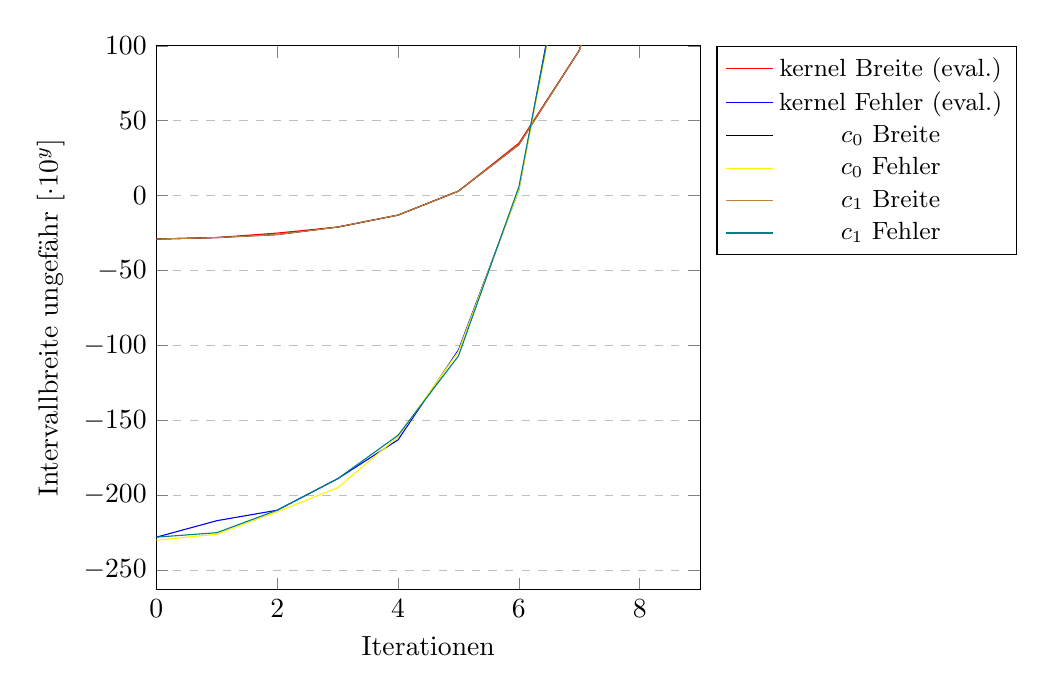
\begin{tikzpicture}
    \begin{axis}[
        width=0.7\textwidth,
        height=0.7\textwidth,
        xlabel={Iterationen},
        ylabel={Intervallbreite ungefähr $[\cdot 10^y ]$},
        legend pos=north west,
        xmin=0,xmax=9,
        ymax=100,
        ymajorgrids=true,
        grid style=dashed,
        legend pos=outer north east,
        cycle list name=color list
    ]
    
    \addplot
        coordinates {
 (0,-29)
 (1,-28)
 (2,-25)
 (3,-21)
 (4,-13)
 (5,03)
 (6,035)
 (7,097)
 (8,0223)
        };
        \addlegendentry{\small{kernel Breite (eval.)}}
    
    \addplot
        coordinates {
  (0,-228)
 (1,-217)
 (2,-210)
 (3,-189)
 (4,-163)
 (5,-103)
 (6,4)
 (7,220)
        };
        \addlegendentry{\small{kernel Fehler (eval.)}}
       
    
    \addplot
        coordinates {
 (0,-29)
 (1,-28)
 (2,-26)
 (3,-21)
 (4,-13)
 (5,03)
 (6,034)
 (7,097)
 (8,0223)
        };
        \addlegendentry{\small{$c_0$ Breite}}
        
    \addplot
        coordinates {
  (0,-230)
 (1,-226)
 (2,-211)
 (3,-195)
 (4,-161)
 (5,-104)
 (6,4)
 (7,212)
 (8,631)
        };
        \addlegendentry{\small{$c_0$ Fehler}}
    
        \addplot
        coordinates {
 (0,-29)
 (1,-28)
 (2,-26)
 (3,-21)
 (4,-13)
 (5,03)
 (6,034)
 (7,097)
 (8,0223)
        };
        \addlegendentry{\small{$c_1$ Breite}}
    
        \addplot
        coordinates {
   (0,-228)
 (1,-225)
 (2,-210)
 (3,-189)
 (4,-160)
 (5,-107)
 (6,6)
 (7,214)
        };
        \addlegendentry{\small{$c_1$ Fehler}}
    
    
    \end{axis}
    \end{tikzpicture}
    \caption{$x_0 = [0 \pm 0] + [0.5 \pm \varepsilon] \cdot \lambda,\  \lambda \in [1 \pm 0]$}
    \label{fig:tm4}
\end{figure}
% 
\begin{figure}[ht]
    \centering
    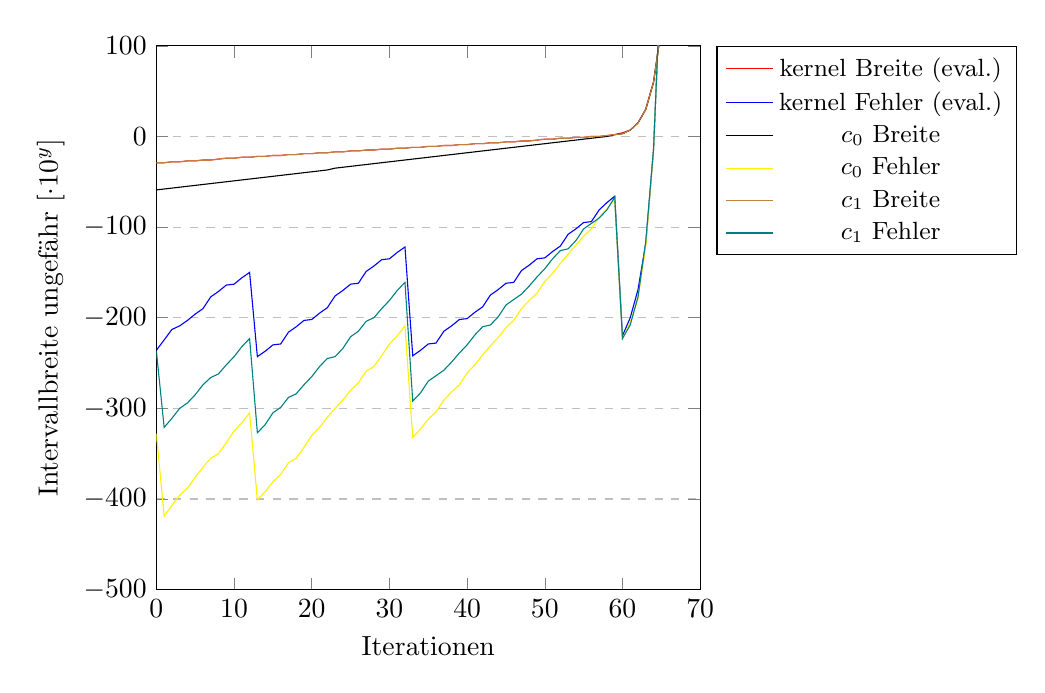
\begin{tikzpicture}
    \begin{axis}[
        width=0.7\textwidth,
        height=0.7\textwidth,
        xlabel={Iterationen},
        ylabel={Intervallbreite ungefähr $[\cdot 10^y ]$},
        legend pos=north west,
        xmin=0,xmax=70,
        ymax=100,ymin=-500,
        ymajorgrids=true,
        grid style=dashed,
        legend pos=outer north east,
        cycle list name=color list
    ]
    
    \addplot
        coordinates {
 (0,-29)
 (1,-29)
 (2,-28)
 (3,-28)
 (4,-27)
 (5,-27)
 (6,-26)
 (7,-26)
 (8,-25)
 (9,-24)
 (10,-24)
 (11,-23)
 (12,-23)
 (13,-22)
 (14,-22)
 (15,-21)
 (16,-21)
 (17,-20)
 (18,-20)
 (19,-19)
 (20,-19)
 (21,-18)
 (22,-18)
 (23,-17)
 (24,-17)
 (25,-16)
 (26,-16)
 (27,-15)
 (28,-15)
 (29,-14)
 (30,-14)
 (31,-13)
 (32,-13)
 (33,-12)
 (34,-12)
 (35,-11)
 (36,-11)
 (37,-10)
 (38,-10)
 (39,-9)
 (40,-9)
 (41,-8)
 (42,-8)
 (43,-7)
 (44,-7)
 (45,-6)
 (46,-6)
 (47,-5)
 (48,-5)
 (49,-4)
 (50,-3)
 (51,-3)
 (52,-2)
 (53,-2)
 (54,-1)
 (55,-1)
 (56,0)
 (57,0)
 (58,01)
 (59,02)
 (60,04)
 (61,07)
 (62,015)
 (63,030)
 (64,060)
 (65,0120)
        };
        \addlegendentry{\small{kernel Breite (eval.)}}
    
    \addplot
        coordinates {
  (0,-236)
 (2,-213)
 (3,-209)
 (4,-203)
 (5,-196)
 (6,-190)
 (7,-177)
 (8,-171)
 (9,-164)
 (10,-163)
 (11,-156)
 (12,-150)
 (13,-243)
 (14,-237)
 (15,-230)
 (16,-229)
 (17,-216)
 (18,-210)
 (19,-203)
 (20,-202)
 (21,-195)
 (22,-189)
 (23,-176)
 (24,-170)
 (25,-163)
 (26,-162)
 (27,-149)
 (28,-143)
 (29,-136)
 (30,-135)
 (31,-128)
 (32,-122)
 (33,-242)
 (34,-236)
 (35,-229)
 (36,-228)
 (37,-215)
 (38,-209)
 (39,-202)
 (40,-201)
 (41,-194)
 (42,-188)
 (43,-175)
 (44,-169)
 (45,-162)
 (46,-161)
 (47,-148)
 (48,-142)
 (49,-135)
 (50,-134)
 (51,-127)
 (52,-121)
 (53,-108)
 (54,-102)
 (55,-95)
 (56,-94)
 (57,-81)
 (58,-73)
 (59,-66)
 (60,-220)
 (61,-200)
 (62,-169)
 (63,-118)
 (64,-14)
 (65,191)
        };
        \addlegendentry{\small{kernel Fehler (eval.)}}
       
    
    \addplot
        coordinates {
 (0,-59)
 (1,-58)
 (2,-57)
 (3,-56)
 (4,-55)
 (5,-54)
 (6,-53)
 (7,-52)
 (8,-51)
 (9,-50)
 (10,-49)
 (11,-48)
 (12,-47)
 (13,-46)
 (14,-45)
 (15,-44)
 (16,-43)
 (17,-42)
 (18,-41)
 (19,-40)
 (20,-39)
 (21,-38)
 (22,-37)
 (23,-35)
 (24,-34)
 (25,-33)
 (26,-32)
 (27,-31)
 (28,-30)
 (29,-29)
 (30,-28)
 (31,-27)
 (32,-26)
 (33,-25)
 (34,-24)
 (35,-23)
 (36,-22)
 (37,-21)
 (38,-20)
 (39,-19)
 (40,-18)
 (41,-17)
 (42,-16)
 (43,-15)
 (44,-14)
 (45,-13)
 (46,-12)
 (47,-11)
 (48,-10)
 (49,-9)
 (50,-8)
 (51,-7)
 (52,-6)
 (53,-5)
 (54,-4)
 (55,-3)
 (56,-2)
 (57,-1)
 (58,0)
 (59,02)
 (60,03)
 (61,07)
 (62,015)
 (63,030)
 (64,060)
 (65,0119)
        };
        \addlegendentry{\small{$c_0$ Breite}}
        
    \addplot
        coordinates {
  (0,-328)
 (1,-419)
 (2,-407)
 (3,-396)
 (4,-388)
 (5,-376)
 (6,-365)
 (7,-355)
 (8,-350)
 (9,-338)
 (10,-325)
 (11,-316)
 (12,-305)
 (13,-401)
 (14,-392)
 (15,-381)
 (16,-373)
 (17,-360)
 (18,-355)
 (19,-343)
 (20,-330)
 (21,-321)
 (22,-310)
 (23,-300)
 (24,-291)
 (25,-280)
 (26,-272)
 (27,-259)
 (28,-254)
 (29,-242)
 (30,-229)
 (31,-220)
 (32,-209)
 (33,-332)
 (34,-323)
 (35,-312)
 (36,-304)
 (37,-291)
 (38,-282)
 (39,-274)
 (40,-261)
 (41,-252)
 (42,-241)
 (43,-231)
 (44,-222)
 (45,-211)
 (46,-203)
 (47,-190)
 (48,-181)
 (49,-173)
 (50,-160)
 (51,-151)
 (52,-140)
 (53,-130)
 (54,-120)
 (55,-110)
 (56,-102)
 (57,-89)
 (58,-80)
 (59,-69)
 (60,-223)
 (61,-205)
 (62,-179)
 (63,-121)
 (64,-15)
 (65,191)
        };
        \addlegendentry{\small{$c_0$ Fehler}}
    
        \addplot
        coordinates {
 (0,-29)
 (1,-29)
 (2,-28)
 (3,-28)
 (4,-27)
 (5,-27)
 (6,-26)
 (7,-26)
 (8,-25)
 (9,-24)
 (10,-24)
 (11,-23)
 (12,-23)
 (13,-22)
 (14,-22)
 (15,-21)
 (16,-21)
 (17,-20)
 (18,-20)
 (19,-19)
 (20,-19)
 (21,-18)
 (22,-18)
 (23,-17)
 (24,-17)
 (25,-16)
 (26,-16)
 (27,-15)
 (28,-15)
 (29,-14)
 (30,-14)
 (31,-13)
 (32,-13)
 (33,-12)
 (34,-12)
 (35,-11)
 (36,-11)
 (37,-10)
 (38,-10)
 (39,-9)
 (40,-9)
 (41,-8)
 (42,-8)
 (43,-7)
 (44,-7)
 (45,-6)
 (46,-6)
 (47,-5)
 (48,-5)
 (49,-4)
 (50,-3)
 (51,-3)
 (52,-2)
 (53,-2)
 (54,-1)
 (55,-1)
 (56,0)
 (57,0)
 (58,01)
 (59,02)
 (60,03)
 (61,07)
 (62,015)
 (63,030)
 (64,060)
 (65,0119)
        };
        \addlegendentry{\small{$c_1$ Breite}}
    
        \addplot
        coordinates {
   (0,-237)
 (1,-321)
 (2,-311)
 (3,-300)
 (4,-294)
 (5,-285)
 (6,-274)
 (7,-266)
 (8,-262)
 (9,-252)
 (10,-243)
 (11,-232)
 (12,-223)
 (13,-327)
 (14,-318)
 (15,-305)
 (16,-299)
 (17,-288)
 (18,-284)
 (19,-274)
 (20,-265)
 (21,-254)
 (22,-245)
 (23,-243)
 (24,-234)
 (25,-221)
 (26,-215)
 (27,-204)
 (28,-200)
 (29,-190)
 (30,-181)
 (31,-170)
 (32,-161)
 (33,-292)
 (34,-283)
 (35,-270)
 (36,-264)
 (37,-258)
 (38,-249)
 (39,-239)
 (40,-230)
 (41,-219)
 (42,-210)
 (43,-208)
 (44,-199)
 (45,-186)
 (46,-180)
 (47,-174)
 (48,-165)
 (49,-155)
 (50,-146)
 (51,-135)
 (52,-126)
 (53,-124)
 (54,-115)
 (55,-102)
 (56,-96)
 (57,-90)
 (58,-81)
 (59,-67)
 (60,-223)
 (61,-208)
 (62,-177)
 (63,-116)
 (64,-14)
 (65,190)

        };
        \addlegendentry{\small{$c_1$ Fehler}}
    
    
    \end{axis}
    \end{tikzpicture}
    \caption{$x_0 = [0.5 \pm 0] + [0 \pm \varepsilon] \cdot \lambda ,\ \lambda \in [1 \pm 0]$}
    \label{fig:tm5}
\end{figure}
% 
\begin{figure}[ht]
    \centering
    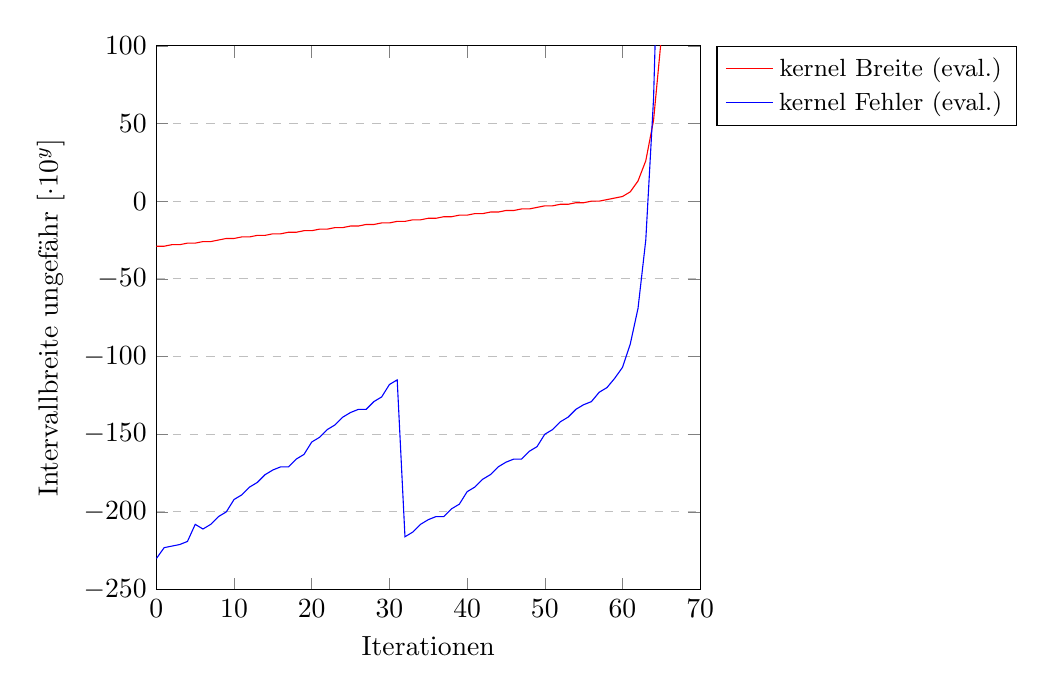
\begin{tikzpicture}
    \begin{axis}[
        width=0.7\textwidth,
        height=0.7\textwidth,
        xlabel={Iterationen},
        ylabel={Intervallbreite ungefähr $[\cdot 10^y ]$},
        legend pos=north west,
        xmin=0,xmax=70,
        ymax=100,ymin=-250,
        ymajorgrids=true,
        grid style=dashed,
        legend pos=outer north east,
        cycle list name=color list
    ]
    
    \addplot
        coordinates {
 (0,-29)
 (1,-29)
 (2,-28)
 (3,-28)
 (4,-27)
 (5,-27)
 (6,-26)
 (7,-26)
 (8,-25)
 (9,-24)
 (10,-24)
 (11,-23)
 (12,-23)
 (13,-22)
 (14,-22)
 (15,-21)
 (16,-21)
 (17,-20)
 (18,-20)
 (19,-19)
 (20,-19)
 (21,-18)
 (22,-18)
 (23,-17)
 (24,-17)
 (25,-16)
 (26,-16)
 (27,-15)
 (28,-15)
 (29,-14)
 (30,-14)
 (31,-13)
 (32,-13)
 (33,-12)
 (34,-12)
 (35,-11)
 (36,-11)
 (37,-10)
 (38,-10)
 (39,-9)
 (40,-9)
 (41,-8)
 (42,-8)
 (43,-7)
 (44,-7)
 (45,-6)
 (46,-6)
 (47,-5)
 (48,-5)
 (49,-4)
 (50,-3)
 (51,-3)
 (52,-2)
 (53,-2)
 (54,-1)
 (55,-1)
 (56,0)
 (57,0)
 (58,01)
 (59,02)
 (60,03)
 (61,06)
 (62,013)
 (63,026)
 (64,052)
 (65,0105)
        };
        \addlegendentry{\small{kernel Breite (eval.)}}
    
    \addplot
        coordinates {
  (0,-230)
 (1,-223)
 (2,-222)
 (3,-221)
 (4,-219)
 (5,-208)
 (6,-211)
 (7,-208)
 (8,-203)
 (9,-200)
 (10,-192)
 (11,-189)
 (12,-184)
 (13,-181)
 (14,-176)
 (15,-173)
 (16,-171)
 (17,-171)
 (18,-166)
 (19,-163)
 (20,-155)
 (21,-152)
 (22,-147)
 (23,-144)
 (24,-139)
 (25,-136)
 (26,-134)
 (27,-134)
 (28,-129)
 (29,-126)
 (30,-118)
 (31,-115)
 (32,-216)
 (33,-213)
 (34,-208)
 (35,-205)
 (36,-203)
 (37,-203)
 (38,-198)
 (39,-195)
 (40,-187)
 (41,-184)
 (42,-179)
 (43,-176)
 (44,-171)
 (45,-168)
 (46,-166)
 (47,-166)
 (48,-161)
 (49,-158)
 (50,-150)
 (51,-147)
 (52,-142)
 (53,-139)
 (54,-134)
 (55,-131)
 (56,-129)
 (57,-123)
 (58,-120)
 (59,-114)
 (60,-107)
 (61,-92)
 (62,-69)
 (63,-25)
 (64,66)
 (65,241)
        };
        \addlegendentry{\small{kernel Fehler (eval.)}}
      
    
    \end{axis}
    \end{tikzpicture}
    \caption{$x_0 = [0.5 \pm \varepsilon]$}
    \label{fig:tm6}
\end{figure}
%
\begin{figure}[ht]
    \centering
    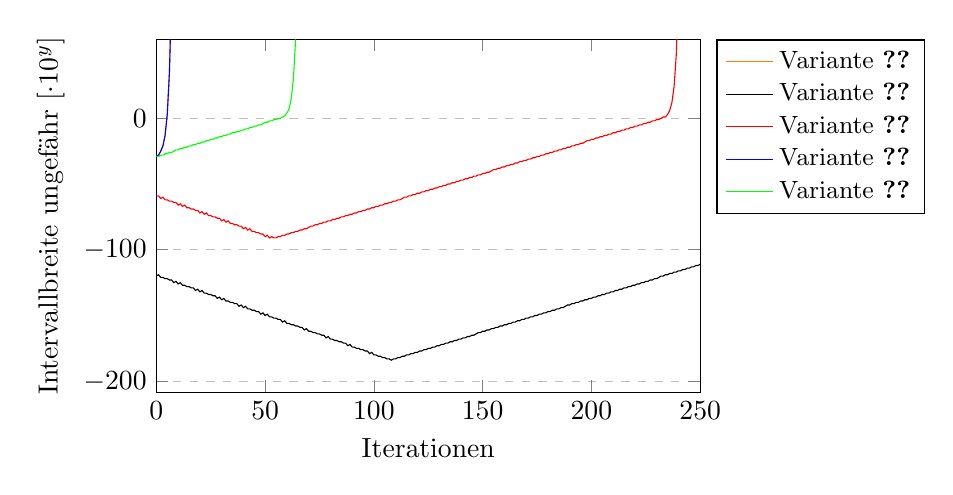
\begin{tikzpicture}
    \begin{axis}[
        width=0.7\textwidth,
        height=0.5\textwidth,
        xlabel={Iterationen},
        ylabel={Intervallbreite ungefähr $[\cdot 10^y ]$},
        legend pos=north west,
        xmin=0,xmax=250,
        ymax=60,
        ymajorgrids=true,
        grid style=dashed,
        legend pos=outer north east
    ]
    
    \addplot[
        color=orange,
        ]
        coordinates {
    (0,-29)
(1,-28)
(2,-25)
(3,-21)
(4,-13)
(5,03)
(6,35)
(7,97)
(8,223)
        };
        \addlegendentry{\small{Variante \ref{tm1}}}
    
    \addplot[
        color=black,
        ]
        coordinates {
    (0,-120) (1,-119) (2,-121) (3,-121) (4,-122) (5,-122) (6,-123) (7,-123) (8,-125) (9,-124) (10,-126) (11,-125) (12,-127) (13,-127) (14,-128) (15,-128) (16,-129) (17,-129) (18,-131) (19,-130) (20,-132) (21,-131) (22,-133) (23,-133) (24,-134) (25,-134) (26,-135) (27,-135) (28,-137) (29,-136) (30,-138) (31,-137) (32,-139) (33,-139) (34,-140) (35,-140) (36,-141) (37,-141) (38,-143) (39,-142) (40,-144) (41,-143) (42,-145) (43,-145) (44,-146) (45,-146) (46,-147) (47,-147) (48,-149) (49,-148) (50,-150) (51,-149) (52,-151) (53,-151) (54,-152) (55,-152) (56,-153) (57,-153) (58,-155) (59,-154) (60,-156) (61,-156) (62,-157) (63,-157) (64,-158) (65,-158) (66,-159) (67,-159) (68,-161) (69,-160) (70,-162) (71,-162) (72,-163) (73,-163) (74,-164) (75,-164) (76,-165) (77,-165) (78,-167) (79,-166) (80,-168) (81,-168) (82,-169) (83,-169) (84,-170) (85,-170) (86,-171) (87,-171) (88,-173) (89,-172) (90,-174) (91,-174) (92,-175) (93,-175) (94,-176) (95,-176) (96,-177) (97,-177) (98,-179) (99,-178) (100,-180) (101,-180) (102,-181) (103,-181) (104,-182) (105,-182) (106,-183) (107,-183) (108,-184) (109,-183) (110,-183) (111,-182) (112,-182) (113,-181) (114,-181) (115,-180) (116,-180) (117,-179) (118,-179) (119,-178) (120,-178) (121,-177) (122,-177) (123,-176) (124,-176) (125,-175) (126,-175) (127,-174) (128,-174) (129,-173) (130,-173) (131,-172) (132,-172) (133,-171) (134,-171) (135,-170) (136,-170) (137,-169) (138,-169) (139,-168) (140,-168) (141,-167) (142,-167) (143,-166) (144,-166) (145,-165) (146,-165) (147,-164) (148,-163) (149,-163) (150,-162) (151,-162) (152,-161) (153,-161) (154,-160) (155,-160) (156,-159) (157,-159) (158,-158) (159,-158) (160,-157) (161,-157) (162,-156) (163,-156) (164,-155) (165,-155) (166,-154) (167,-154) (168,-153) (169,-153) (170,-152) (171,-152) (172,-151) (173,-151) (174,-150) (175,-150) (176,-149) (177,-149) (178,-148) (179,-148) (180,-147) (181,-147) (182,-146) (183,-146) (184,-145) (185,-145) (186,-144) (187,-144) (188,-143) (189,-142) (190,-142) (191,-141) (192,-141) (193,-140) (194,-140) (195,-139) (196,-139) (197,-138) (198,-138) (199,-137) (200,-137) (201,-136) (202,-136) (203,-135) (204,-135) (205,-134) (206,-134) (207,-133) (208,-133) (209,-132) (210,-132) (211,-131) (212,-131) (213,-130) (214,-130) (215,-129) (216,-129) (217,-128) (218,-128) (219,-127) (220,-127) (221,-126) (222,-126) (223,-125) (224,-125) (225,-124) (226,-124) (227,-123) (228,-123) (229,-122) (230,-122) (231,-121) (232,-120) (233,-120) (234,-119) (235,-119) (236,-118) (237,-118) (238,-117) (239,-117) (240,-116) (241,-116) (242,-115) (243,-115) (244,-114) (245,-114) (246,-113) (247,-113) (248,-112) (249,-112) (250,-111)
        };
        \addlegendentry{\small{Variante \ref{tm2}}}
        
    \addplot[
        color=red,
        ]
        coordinates {
    (0,-59) (1,-59) (2,-61) (3,-60) (4,-62) (5,-62) (6,-63) (7,-63) (8,-64) (9,-64) (10,-66) (11,-65) (12,-67) (13,-66) (14,-68) (15,-68) (16,-69) (17,-69) (18,-70) (19,-70) (20,-72) (21,-71) (22,-73) (23,-72) (24,-74) (25,-74) (26,-75) (27,-75) (28,-76) (29,-76) (30,-78) (31,-77) (32,-79) (33,-78) (34,-80) (35,-80) (36,-81) (37,-81) (38,-82) (39,-82) (40,-84) (41,-83) (42,-85) (43,-84) (44,-86) (45,-86) (46,-87) (47,-87) (48,-88) (49,-88) (50,-90) (51,-89) (52,-91) (53,-90) (54,-91) (55,-91) (56,-90) (57,-90) (58,-89) (59,-89) (60,-88) (61,-88) (62,-87) (63,-87) (64,-86) (65,-86) (66,-85) (67,-85) (68,-84) (69,-84) (70,-83) (71,-82) (72,-82) (73,-81) (74,-81) (75,-80) (76,-80) (77,-79) (78,-79) (79,-78) (80,-78) (81,-77) (82,-77) (83,-76) (84,-76) (85,-75) (86,-75) (87,-74) (88,-74) (89,-73) (90,-73) (91,-72) (92,-72) (93,-71) (94,-71) (95,-70) (96,-70) (97,-69) (98,-69) (99,-68) (100,-68) (101,-67) (102,-67) (103,-66) (104,-66) (105,-65) (106,-65) (107,-64) (108,-64) (109,-63) (110,-63) (111,-62) (112,-62) (113,-61) (114,-60) (115,-60) (116,-59) (117,-59) (118,-58) (119,-58) (120,-57) (121,-57) (122,-56) (123,-56) (124,-55) (125,-55) (126,-54) (127,-54) (128,-53) (129,-53) (130,-52) (131,-52) (132,-51) (133,-51) (134,-50) (135,-50) (136,-49) (137,-49) (138,-48) (139,-48) (140,-47) (141,-47) (142,-46) (143,-46) (144,-45) (145,-45) (146,-44) (147,-44) (148,-43) (149,-43) (150,-42) (151,-42) (152,-41) (153,-41) (154,-40) (155,-39) (156,-39) (157,-38) (158,-38) (159,-37) (160,-37) (161,-36) (162,-36) (163,-35) (164,-35) (165,-34) (166,-34) (167,-33) (168,-33) (169,-32) (170,-32) (171,-31) (172,-31) (173,-30) (174,-30) (175,-29) (176,-29) (177,-28) (178,-28) (179,-27) (180,-27) (181,-26) (182,-26) (183,-25) (184,-25) (185,-24) (186,-24) (187,-23) (188,-23) (189,-22) (190,-22) (191,-21) (192,-21) (193,-20) (194,-20) (195,-19) (196,-19) (197,-18) (198,-17) (199,-17) (200,-16) (201,-16) (202,-15) (203,-15) (204,-14) (205,-14) (206,-13) (207,-13) (208,-12) (209,-12) (210,-11) (211,-11) (212,-10) (213,-10) (214,-9) (215,-9) (216,-8) (217,-8) (218,-7) (219,-7) (220,-6) (221,-6) (222,-5) (223,-5) (224,-4) (225,-4) (226,-3) (227,-3) (228,-2) (229,-2) (230,-1) (231,-1) (232,00) (233,01) (234,01) (235,03) (236,06) (237,12) (238,24) (239,48) (240,96)
        };
        \addlegendentry{\small{Variante \ref{tm3}}}
    
    
    \addplot[
        color=blue,
        ]
        coordinates {
    (0,-29) (1,-28) (2,-25) (3,-21) (4,-13) (5,03) (6,35) (7,97)
        };
        \addlegendentry{\small{Variante \ref{tm4}}}
    
    \addplot[
        color=green,
        ]
        coordinates {
    (0,-29) (1,-29) (2,-28) (3,-28) (4,-27) (5,-27) (6,-26) (7,-26) (8,-25) (9,-24) (10,-24) (11,-23) (12,-23) (13,-22) (14,-22) (15,-21) (16,-21) (17,-20) (18,-20) (19,-19) (20,-19) (21,-18) (22,-18) (23,-17) (24,-17) (25,-16) (26,-16) (27,-15) (28,-15) (29,-14) (30,-14) (31,-13) (32,-13) (33,-12) (34,-12) (35,-11) (36,-11) (37,-10) (38,-10) (39,-9) (40,-9) (41,-8) (42,-8) (43,-7) (44,-7) (45,-6) (46,-6) (47,-5) (48,-5) (49,-4) (50,-3) (51,-3) (52,-2) (53,-2) (54,-1) (55,-1) (56,00) (57,00) (58,01) (59,02) (60,04) (61,07) (62,15) (63,30) (64,60)
        };
        \addlegendentry{\small{Variante \ref{tm5}}}
                                      
    
    
    
    
    \end{axis}
    \end{tikzpicture}
    \caption{Größenordnung der Breite des Kernintervalls bei der Berechnung von $x_{250}$ mit Sweeping square\_only mit unterschiedlichen Definitionen des Taylormodells für $x_0$}
    \label{fig:strategy2}
\end{figure}


%% ==============================
\label{ch:Evaluierung:sec:zusammenfassung}


%%% Local Variables: 
%%% mode: latex
%%% TeX-master: "thesis"
%%% End: 

        % Evaluation
%% zusammenf.tex
%% $Id: zusammenf.tex 61 2012-05-03 13:58:03Z bless $
%%

\chapter{Diskussion}
\label{ch:fazit}
%% ==============================

\chapter{Ausblick}
In dieser Arbeit wurde eine grundlegende Implementierung für das Rechnen mit nichtlinearen Taylormodellen auf den reellen Zahlen beschrieben und angefertigt. An verschiedenen Stellen ist es jedoch möglich und teils notwendig, die Arbeit fortzuführen

\section{Partitionierung}

\section{Laufzeitoptimierung}

\section{Schnittstellen}


%%% Local Variables: 
%%% mode: latex
%%% TeX-master: "thesis"
%%% End: 
   	  % Diskussion und Ausblick

%% ++++++++++++++++++++++++++++++++++++++++++
%% Anhang
%% ++++++++++++++++++++++++++++++++++++++++++



%\include{anhang_b}

%% ++++++++++++++++++++++++++++++++++++++++++
%% Literatur
%% ++++++++++++++++++++++++++++++++++++++++++
%  mit dem Befehl \nocite werden auch nicht 
%  zitierte Referenzen abgedruckt

\cleardoublepage    
\phantomsection  
\addcontentsline{toc}{chapter}{\bibname}
%%
%\nocite{*} % nur angeben, wenn auch nicht im Text zitierte Quellen 
           % erscheinen sollen
\bibliographystyle{itmabbrv} % mit abgekürzten Vornamen der Autoren
%\bibliographystyle{gerplain} % abbrvnat unsrtnat
% spezielle Zitierstile: Labels mit vier Buchstaben und Jahreszahl
%\bibliographystyle{itmalpha}  % ausgeschriebene Vornamen der Autoren
\bibliography{thesis}
\chapter{Anhang}

\section*{Algorithmen für Geobuckets}
\begin{algorithm}
\SetAlgoLined
\SetKwInOut{Input}{Eingabe}
\SetKwInOut{Output}{Ausgabe}
\Input{Polynome $p, q$ mit Monomen $m_{p_i}$ und $m_{q_j}$, wobei $i = \#p$ und $j = \#q$}
\Output{Polynom $p'$ mit geordneten Monomen}
$n \gets \#p, k\gets \#q$ \\
$buckets$ mit Platz geom. wachsender Größe anlegen: $\{2k, 4k, ..., 2^{\lceil log_2(n)\rceil -1 }k\}$\\
$i\gets 0 $\\
\While(\Comment*[f]{Bis jedes Monom aus $q$ betrachtet wurde}){$i < n$}{
    $p' \gets m_{p_i} \cdot q$\\
    \uIf{$i < (n-1)$}{
        $p' \gets p' + m_{p_{i+1}} \cdot q$\\
    }
    $i\gets i+2$\\
   $j\gets 0 $\\ 
    \While(\Comment*[f]{Sammle alle Buckets ein und speichere in $p'$}){$buckets[j]\neq \emptyset$}{
        $p' \gets p' + buckets[j]$\Comment*{Polynome gleicher Größe werden addiert}
        $buckets[j] \gets [\ ]$\\
        $j\gets j+1 $\\ 
    }
    \uIf(\Comment*[f]{Wurde $q$ nicht komplett betrachtet}){$i < n$}{
        $buckets[j] \gets p'$\Comment*{Speichere $p'$ im aktuell leeren Bucket $j$}
        $p' \gets 0$ \Comment*{Leere $p'$ für eine neue Iteration vorbereiten}
    }
    
}
\ForEach(\Comment*[f]{Merge aller Buckets ins Polynom}){$bucket \in buckets$}{
    $p' \gets p' + bucket$\Comment*{vom kleinsten zum größten}
}


\Return $p'$

 \caption{Polynommultipliaktion mit Geobuckets}
 \label{algo:mult}
\end{algorithm}


\begin{algorithm}[H]
\SetAlgoLined
\label{algo:add}
\SetKwInOut{Input}{Eingabe}
\SetKwInOut{Output}{Ausgabe}
\Input{Polynome $p, q$ mit Monomen $m_{p_i}$ und $m_{q_j}$, wobei $i = \#p$ und $j = \#q$}
\Output{Polynom $p'$ mit geordneten Monomen}
$i \gets 0, j \gets 0$ \\
\While(\Comment*[f]{Solange ein Polynom nicht komplett betrachtet wurde}){$i < \#p$ \textbf{and} $j  < \#q$} {
    \uIf{$m_{p_i} \succ m_{q_j}$}{
        $p' \gets p' + m_{p_i}$\\
        $i \gets i+1 $\\
    }
    \uElseIf{$m_{q_j} \succ m_{p_i}$}{
        $p' \gets p' + m_{q_j}$\\
        $j \gets j+1 $\\
    }
    \uElse(\Comment*[f]{Beide Monome haben dieselben Variablen}){
        $p' \gets p' + (m_{q_j} + m_{p_i})$\\
        $i \gets i+1; j \gets j +1 $\\
    }
}
\If{$i < \#p$ \textbf{or} $j  < \#q$}{
Füge den Rest zu $p$ hinzu
}

\Return $p$

 \caption{Addition zweier geordneter Polynome}
\end{algorithm}


\Abbildungps{tbh}{.9}{img/7iter_w_sweep.pdf}{fig:7iter}{H\e non-Abbildung: Mehrere Iterationen mit Farbkodierung}{Mehrere Iterationen mit Farbkodierung}

\section*{Details der Implementierung}

\begin{lstlisting}[language=JSON, caption=Bespielkonfiguration,captionpos=b, label=list:config]
 [
  {
    "comment": "Error 100",
    "rel": 1,
    "linear": 0,
    "keep": 2,
    "error_in_lambda": true,
    "strategy": "SQUARE_ONLY",
    "iter": 1000,
    "prec": 50,
    "error": 1000,
    "decimals": 20,
    "sweep_to": 2,
    "micro_thresh": 1,
    "macro_thresh": 1,
    "a": 1.4,
    "b": 0.3,
    "support_space": [
      {
        "point": false,
        "mid": "0",
        "rad": "e"
      },
      {
        "point": false,
        "mid": "0",
        "rad": "e"
      }
    ],
    "x": {
      "kernel": {
        "point": true,
        "mid": "1",
        "rad": "0"
      },
      "monomials": [
        {
          "point": true,
          "mid": "1",
          "rad": "0",
          "lambdas": [{
            "exp": 1,
            "index": 0
          }]
        }
      ]
    },
    "y": {
      "kernel": {
        "point": true,
        "mid": "0.1",
        "rad": "0"
      },
      "monomials": [
        {
          "point": true,
          "mid": "1",
          "rad": "0",
          "lambdas": [{
            "exp": 1,
            "index": 1
          }]
        }
      ]
    }
  }
]
\end{lstlisting}

%% ++++++++++++++++++++++++++++++++++++++++++
%% Index
%% ++++++++++++++++++++++++++++++++++++++++++
\ifnotdraft{
\cleardoublepage
\phantomsection
\printindex            % Index, Stichwortverzeichnis
}

 %
 % Die folgende Erklärung ist für Diplomarbeiten Pflicht
 % (siehe Prüfungsordnung), für Studienarbeiten nicht notwendig
 \include{src/erklaerung}
 \blankpage % Leerseite auf Erklärungsrückseite
 
\end{document}
%% end of file
